\documentclass[article,A4,12pt]{llncs}

% Conditional compilation.
% NOTE: If you set fullversionfalse, just compile ONCE so that TOC stays unchanged.
\newif\iffullversion
\fullversiontrue
%\fullversionfalse

\usepackage[T1]{fontenc}
\usepackage{amsmath}
\usepackage{amssymb}
\usepackage{amsfonts}
\usepackage{mathrsfs, bm}

\usepackage{graphicx}
\usepackage{tabularx}
\usepackage{subfig}
\usepackage{epsf,times}
\usepackage{color}
\usepackage{wrapfig}
\usepackage{cases}
\usepackage{multicol}

\usepackage[T1]{fontenc}
%\newcommand{\tmname}[1]{\textsc{#1}}
%\newcommand{\tmop}[1]{\ensuremath{\operatorname{#1}}}
%\newcommand{\tmsamp}[1]{\textsf{#1}}
%\newcommand{\tmtextsc}[1]{{\scshape{#1}}}
%\newcommand{\tmtextsl}[1]{{\slshape{#1}}}
%\newcommand{\tmtexttt}[1]{{\ttfamily{#1}}}

\leftmargin=0.0cm
\oddsidemargin=0.5cm
\evensidemargin=0.5cm
\topmargin=0cm
\textwidth=16.0cm
%\textheight=21.5cm
\textheight=20.0cm
\pagestyle{plain}
\setlength{\columnsep}{20pt}

\def\m{\mathbf{m}}
\def\H{\mathbf{H}}
\def\E{\mathbf{E}}
\newcommand{\vepsi}{{\varepsilon}}
\def\hnorm#1#2{\vert\,#1\,\vert_{#2}}
\newcommand{\R}{{\mathbb R}}
\newcommand{\Sph}{{\mathbb S}}
\def\x{\mathbf{x}}
\def\hvec{\overline{\mathbf{h}}}
\def\evec{\overline{\mathbf{e}}}

\newcommand{ \etal}{\mbox{\emph{et al. }}}

\newcommand\vect[1]{\mbf{#1}}
\newcommand{\mbf}[1]{\mbox{\boldmath$#1$}} 
\newcommand{\RC}[1]{#1 $\times$ #1 $\times$ #1}
\def\um{$\mu$m}
\def\C{$^{\circ}\mathrm{C}$}

\newcommand{\Rmnum}[1]{\expandafter\@slowromancap\romannumeral #1@}

% DEFINITION OF CUSTOM FONT SIZE
\newcommand{\customfontA}{\fontsize{50}{55}\selectfont}
\newcommand{\customfontB}{\fontsize{14.4}{20}\selectfont}
\newcommand{\customfontC}{\fontsize{30}{35}\selectfont}

\DeclareMathAlphabet{\mathpzc}{OT1}{pzc}{m}{it}

\def\clovek#1{\noindent\bgroup\vbox{\noindent#1}\egroup\vskip1em}



\begin{document}



%%%%%%%%%%%%%%%%%%%%%%%%%%%%%%%%%%%%%%%%%%%%%%%%%%%%%%%%%%%%%%%%%%%%%%%%%

\pagestyle{empty}

\vbox{}
\begin{figure}[!ht]
%\hspace{-4mm}

\includegraphics[width=8cm]{imgp/logo.png}
\vspace{18mm}
\end{figure}
\vbox{}
\vspace{0.5cm}


\begin{figure}[!ht]
\begin{center}
\vspace{-6mm}
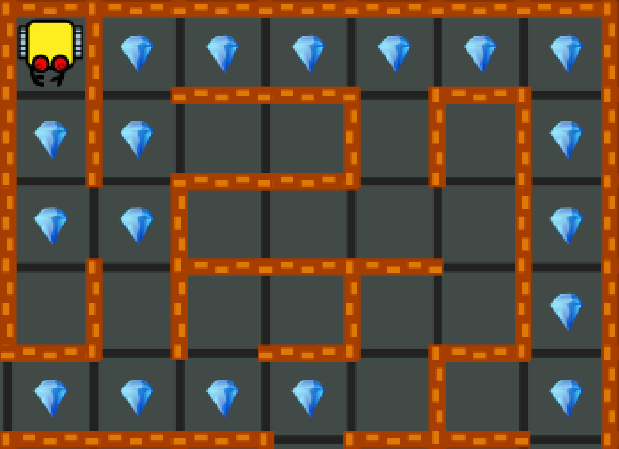
\includegraphics[width=0.26\textheight]{imgk/karel-logo.png}\ \ \ \ \ \ 

\includegraphics[width=0.2\textheight]{imgp/python-logo.png}
\vbox{}
\vspace{-9mm}
\end{center}
\end{figure}
\begin{center}
\vspace{2.8cm}
{\huge \bf Exercises and Solutions}
\end{center}
\vbox{}
\begin{center}
\iffullversion
\else
\vspace{2mm}
\centerline{\huge \color{red}{PREVIEW}}
\fi
\vfill
{\large
{\bf Pavel Solin}, University of Nevada, Reno\\
{\bf Salih Dede}, Coral Academy of Science, Reno
}
\end{center}
\newpage
\vbox{}
\vfill
\begin{center}
{
The textbook {\em Intro to Programming with Karel the Robot and Python} that 
comprises this Exercise Book
can be ordered at {\tt http://introtoprogramming.net}. The textbook 
is also available as part of the NCLab course {\em Intro to Programming} 
that can be purchased at {\tt http://introtoprogramming.net}.
Unauthorized copying and sharing is prohibited.
}
\vfill

Copyright 2012 FEMhub Inc. All rights reserved.
\end{center}




\section*{}
\small

\normalsize

\newpage
%{\ }
\setcounter{tocdepth}{2}
\tableofcontents
%\pagestyle{plain}

\newpage

\pagestyle{plain}
\setcounter{page}{1}

%%%%%%%%%%%%%%%%%%%%%%%%%%%%%%%%%%%%%%%%%%%%%%%%%%%%%%%%%%%%%%%%%%%%%%%%%

\part{Karel the Robot}

\setcounter{section}{2}
\section{Clicking Mode}

\subsection{}

{\em Karel is returning from a long walk and his batteries are running out. 
Use the buttons on the left to get him home quickly! }
\begin{figure}[!ht]
\begin{center}
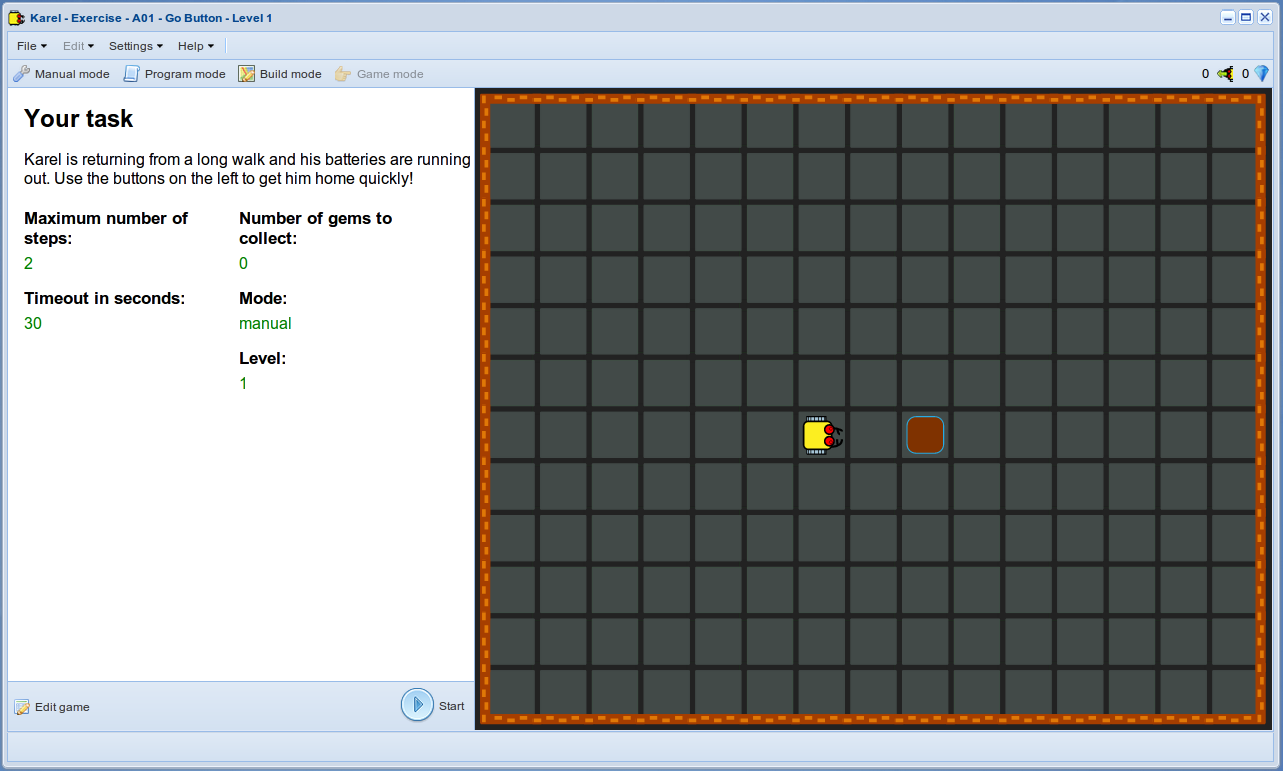
\includegraphics[height=0.4\textwidth]{imgk/a01.png}
\end{center}
\vspace{-4mm}
\caption{In the first exercise you need to help the robot get home.}
\label{fig:a01}
\end{figure}

\noindent
Pressing Start will start 
the exercise, and at this time also the buttons Go, Left, Right, Put and Get appear, 
as shown in Fig. \ref{fig:a01b}.


\begin{figure}[!ht]
\begin{center}
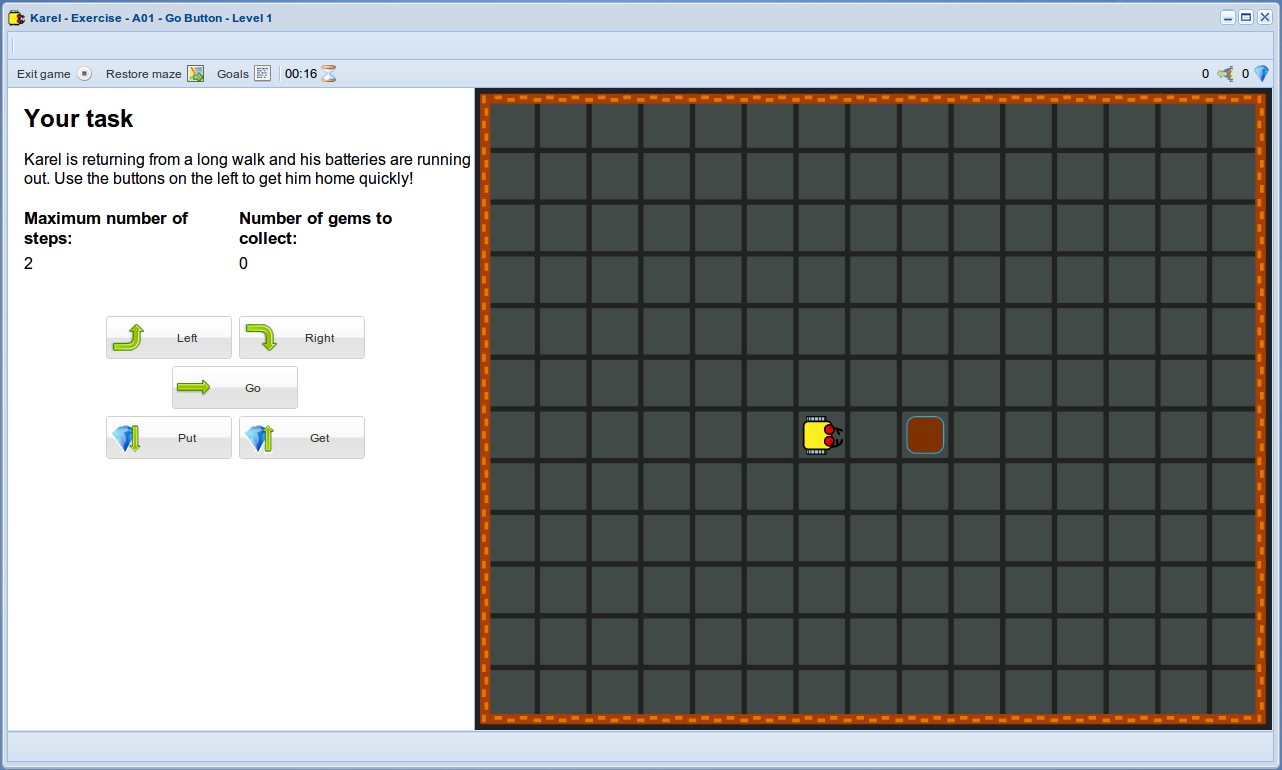
\includegraphics[height=0.4\textwidth]{imgk/a01b.png}
\end{center}
\vspace{-4mm}
\caption{Karel can be guided manually, using five buttons located in the left panel.}
\label{fig:a01b}
\vspace{-10mm}
\end{figure}

\newpage
\subsection{}

{\em Karel is training for Robolympic Games! Your task is to run with 
the robot home as fast as possible. Karel's personal record is four seconds. How fast can you be?}

\begin{figure}[!ht]
\begin{center}
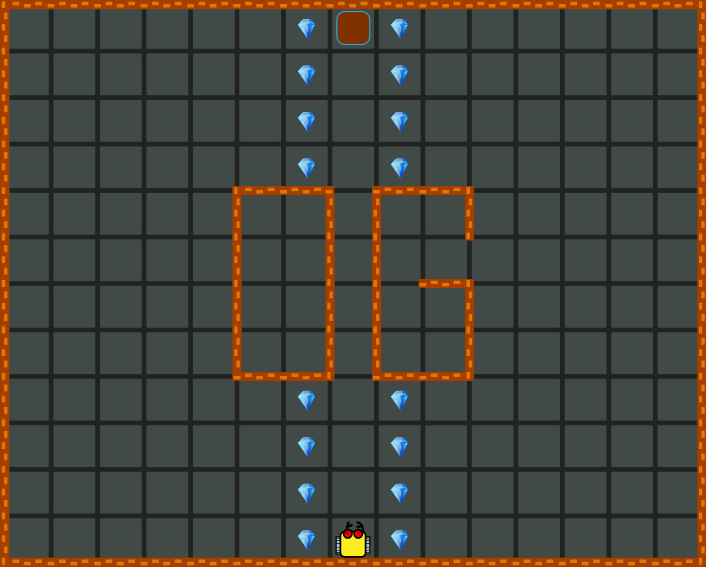
\includegraphics[height=0.4\textwidth]{imgk/a02.png}
\end{center}
\vspace{-4mm}
\caption{Karel is training for Robolympic Games.}
\label{fig:a02}
\vspace{-4mm}
\end{figure}
\noindent

\subsection{}

{\em Today is Karel's lucky day because he is about to find his first gem. 
Use the buttons on the left to help the robot pick up the gem and carry it 
home!}

\begin{figure}[!ht]
\begin{center}
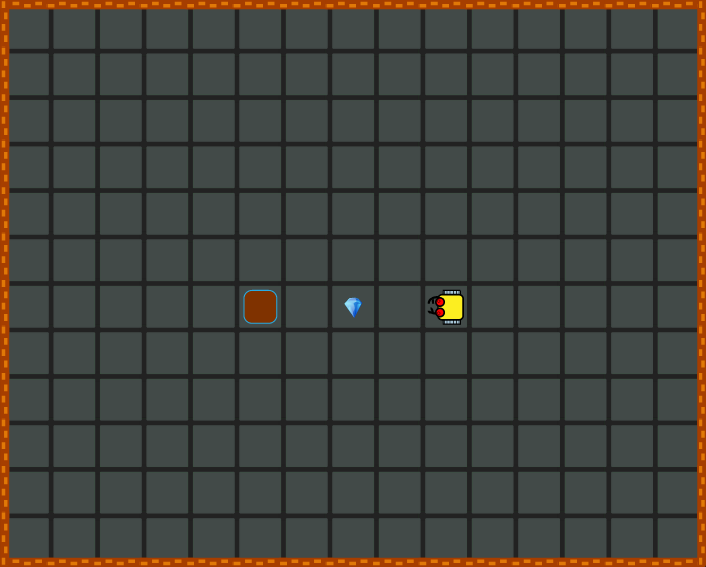
\includegraphics[height=0.4\textwidth]{imgk/a03.png}
\end{center}
\vspace{-4mm}
\caption{Karel is about to find his first gem.}
\label{fig:a03}
\vspace{-1cm}
\end{figure}
\noindent

\subsection{}

{\em It is Robolympic season again! Run home as fast as you can, 
and collect all three gems on the way! Karel's personal record is 10 seconds.}


\begin{figure}[!ht]
\begin{center}
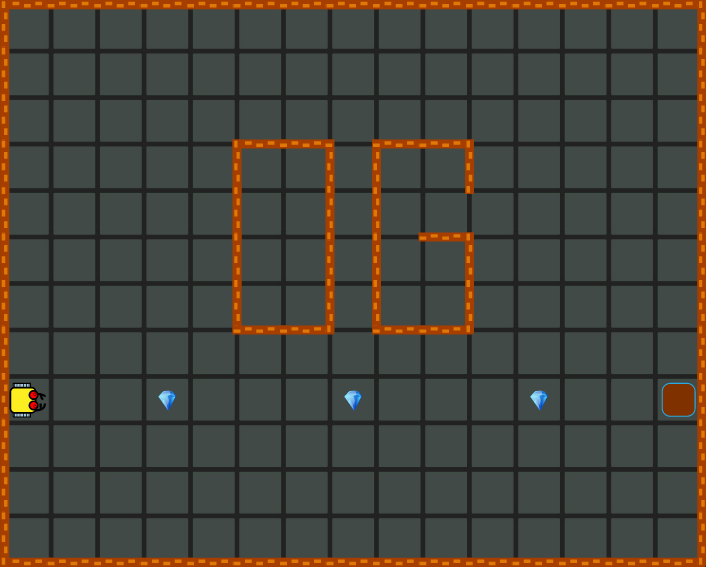
\includegraphics[height=0.4\textwidth]{imgk/a04.png}
\end{center}
\vspace{-4mm}
\caption{Karel's second Robolympic Games.}
\label{fig:a04}
\vspace{-1cm}
\end{figure}
\noindent


\subsection{}

{\em Help the robot collect the gem and return home!}

\begin{figure}[!ht]
\begin{center}
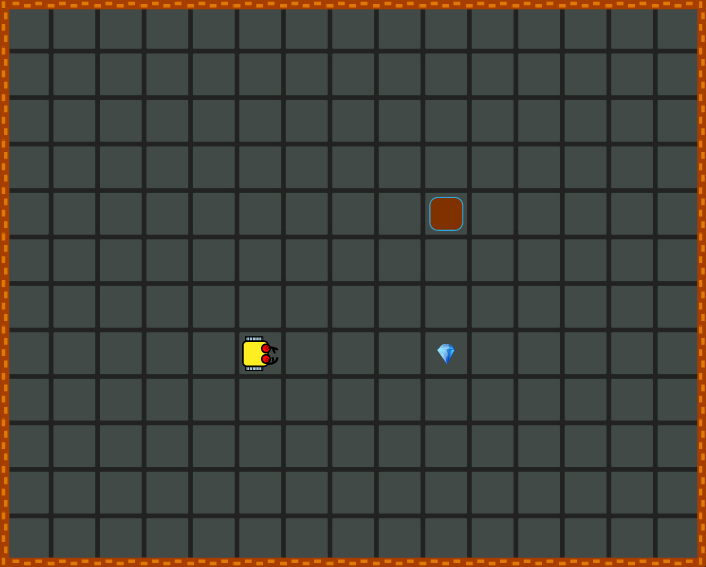
\includegraphics[height=0.4\textwidth]{imgk/a05.png}
\end{center}
\vspace{-4mm}
\caption{Karel is about to learn how to make a left turn.}
\label{fig:a05}
\vspace{-1cm}
\end{figure}
\noindent


\subsection{}

{\em Karel is training for his third Robolympic Games. Run with him around the block and home as fast as possible. He needs to collect at least one gem on the way. Karel's personal record is 16 seconds!}

\begin{figure}[!ht]
\begin{center}
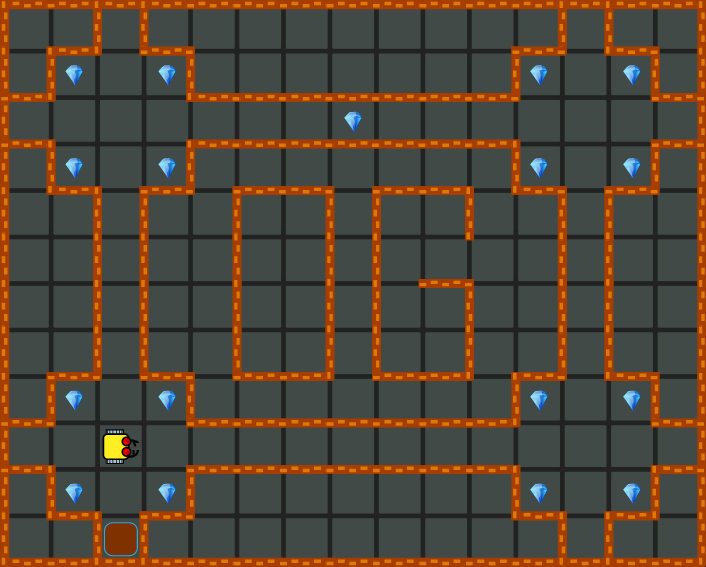
\includegraphics[height=0.4\textwidth]{imgk/a06.png}
\end{center}
\vspace{-4mm}
\caption{Karel's third Robolympic Games.}
\label{fig:a06}
\vspace{-1cm}
\end{figure}
\noindent


\subsection{}

{\em Pick up the two gems and get Karel home!}

\begin{figure}[!ht]
\begin{center}
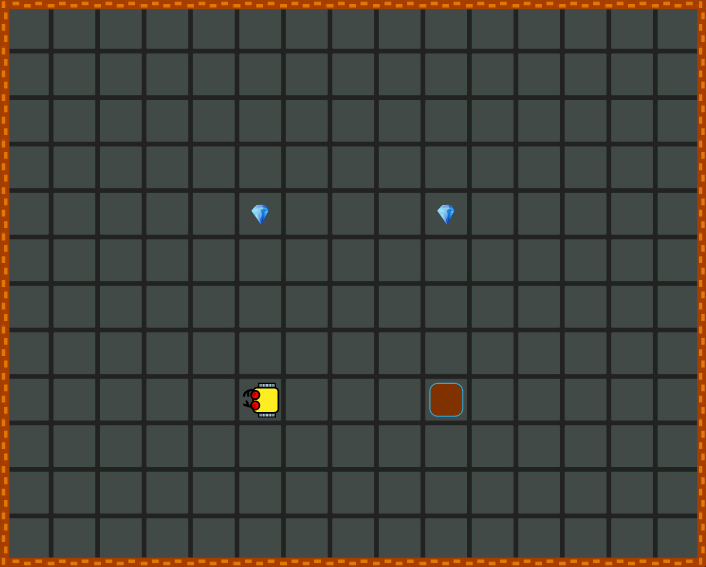
\includegraphics[height=0.4\textwidth]{imgk/a07.png}
\end{center}
\vspace{-4mm}
\caption{Karel needs to collect two gems and get home.}
\label{fig:a07}
\vspace{-1cm}
\end{figure}
\noindent

\subsection{}

{\em Last season of Karel's Robolympics Games is here! The 
robot needs to run home as fast as possible and bring one gem. 
Be careful not to crash, this is a tricky level! Karel's personal record is 26 seconds.}

\begin{figure}[!ht]
\begin{center}
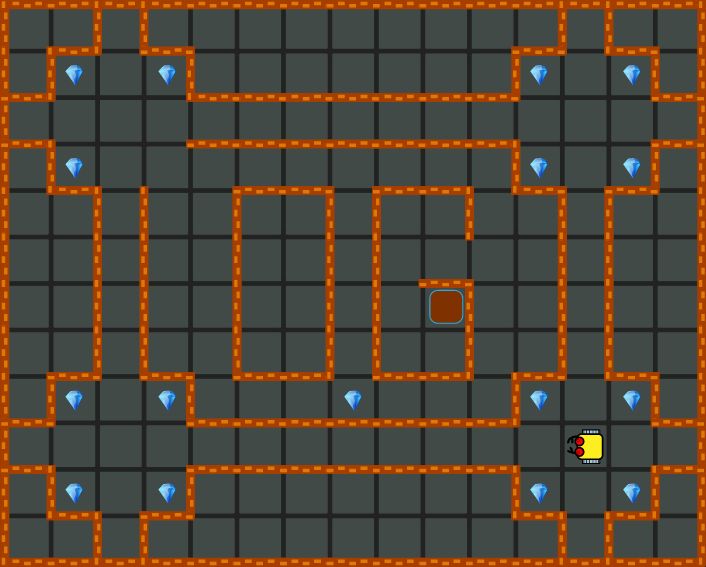
\includegraphics[height=0.4\textwidth]{imgk/a08.png}
\end{center}
\vspace{-4mm}
\caption{Karel's fourth Robolympic Games.}
\label{fig:a08}
\vspace{-4mm}
\end{figure}
\noindent

\subsection{}

{\em​Help Karel collect five gems and get home!}

\begin{figure}[!ht]
\begin{center}
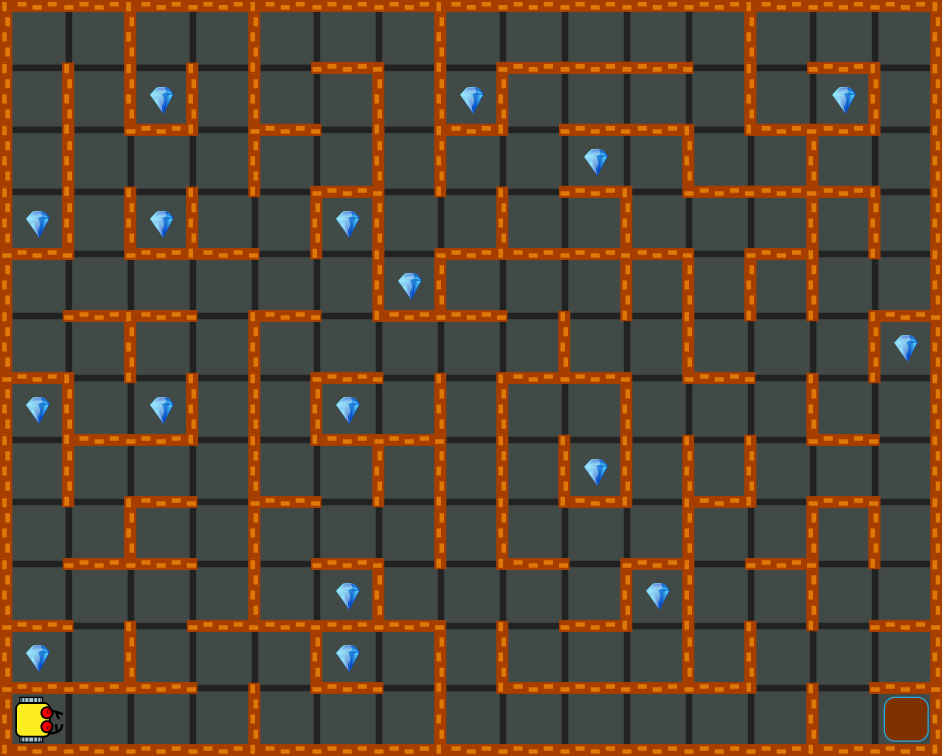
\includegraphics[height=0.4\textwidth]{imgk/a09.png}
\end{center}
\vspace{-4mm}
\caption{Karel needs to collect five gems.}
\label{fig:a09}
\vspace{-4mm}
\end{figure}
\noindent

\subsection{}

{\em This is a true labyrinth and your task is to lead Karel 
home. Remember - think first before going anywhere!}

\begin{figure}[!ht]
\begin{center}
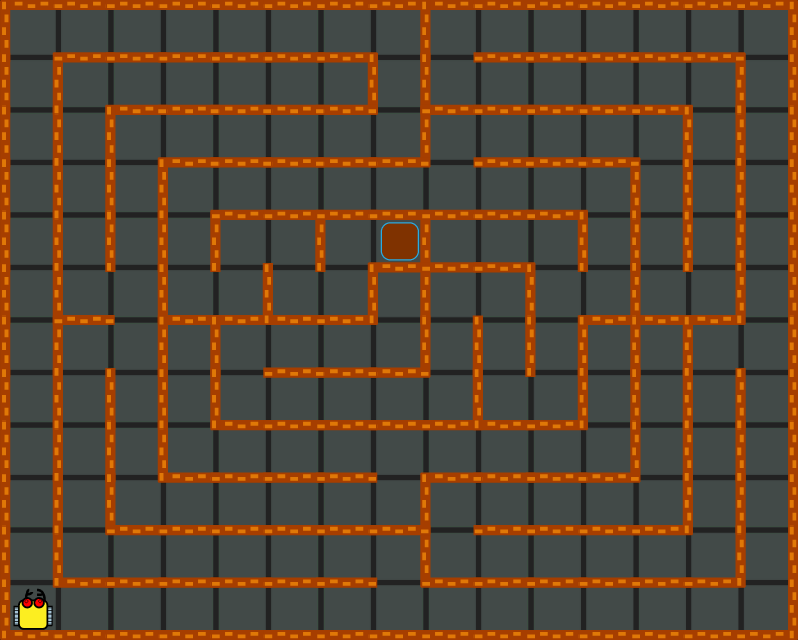
\includegraphics[height=0.4\textwidth]{imgk/a10.png}
\end{center}
\vspace{-4mm}
\caption{Karel needs to find his way home in a labyrinth.}
\label{fig:a10}
\vspace{-4mm}
\end{figure}
\noindent


\subsection{}

{\em Karel discovered an abandoned diamond mine. Use the buttons
on the left to collect all gems and get back home in time!}

\begin{figure}[!ht]
\begin{center}
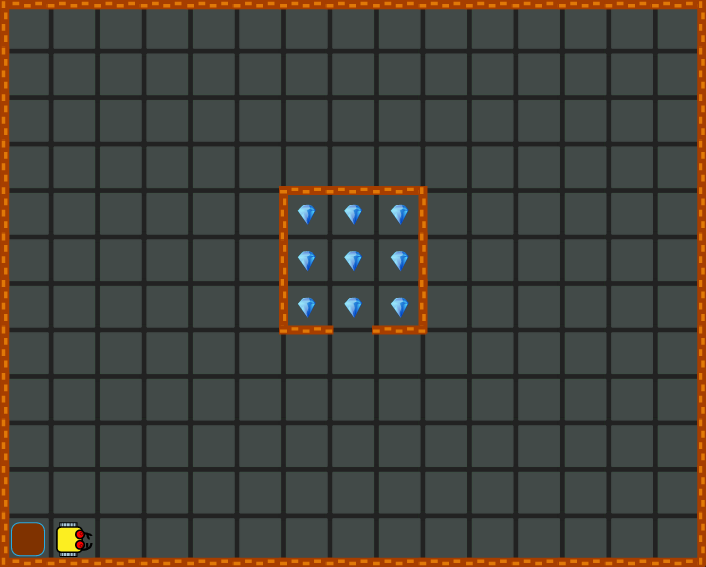
\includegraphics[height=0.4\textwidth]{imgk/a11.png}
\end{center}
\vspace{-4mm}
\caption{Karel found an abandoned diamond mine.}
\label{fig:a11}
\vspace{-10mm}
\end{figure}
\newpage
\noindent

\subsection{}

{\em If gems are piled up, then a number is showing their amount. 
Help Karel collect all gems in this maze and return home!}

\begin{figure}[!ht]
\begin{center}
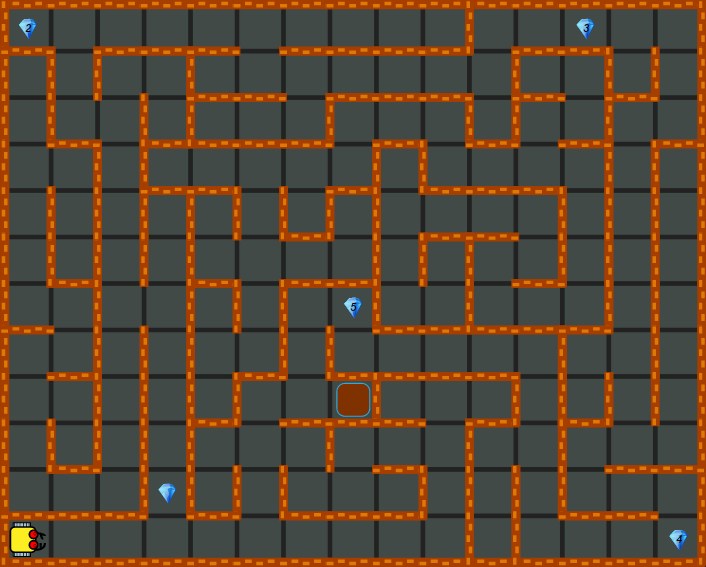
\includegraphics[height=0.4\textwidth]{imgk/a12.png}
\end{center}
\vspace{-4mm}
\caption{If gems are piled up, then a number is showing their amount.}
\label{fig:a12}
\vspace{-10mm}
\end{figure}
\noindent

\subsection{}

{\em Karel has five gems in his bag. Use the buttons on the left to put the gems on the table and 
return home in time!}

\begin{figure}[!ht]
\begin{center}
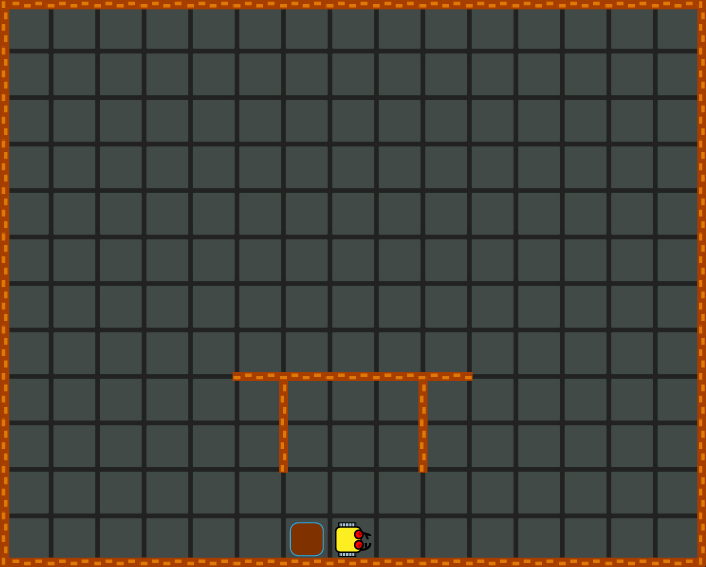
\includegraphics[height=0.4\textwidth]{imgk/a13.png}
\end{center}
\vspace{-4mm}
\caption{Karel needs to put five gems on the table.}
\label{fig:a13}
\vspace{-4mm}
\end{figure}
\noindent

\section{Programming Mode}

\subsection{}

{\em Write a program that gets Karel home! Remember: Always write one command per line.}

\begin{figure}[!ht]
\begin{center}
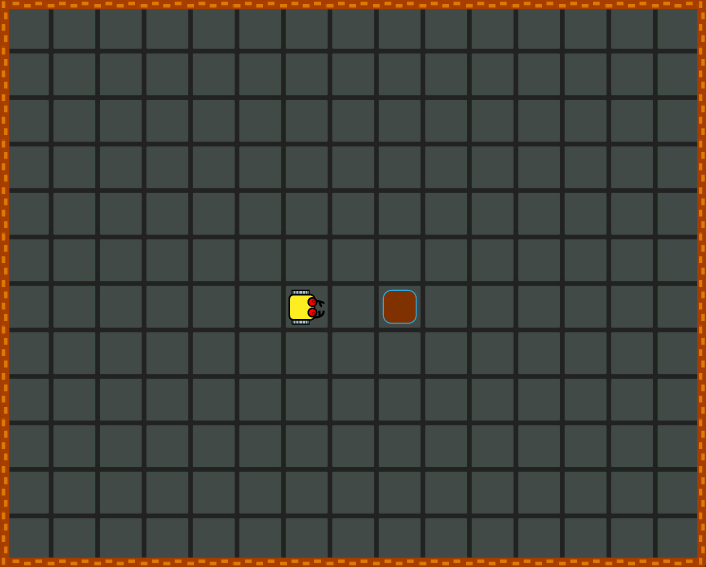
\includegraphics[height=0.4\textwidth]{imgk/b01.png}
\end{center}
\vspace{-4mm}
\caption{Moving Karel forward via the {\tt go} command.}
\label{fig:b01}
\vspace{-4mm}
\end{figure}
\noindent

\subsubsection*{Solution}
\begin{verbatim}
go
go
\end{verbatim}

\newpage
\subsection{}

{\em Write a program for Karel to collect all gems and get home! 

\begin{figure}[!ht]
\begin{center}
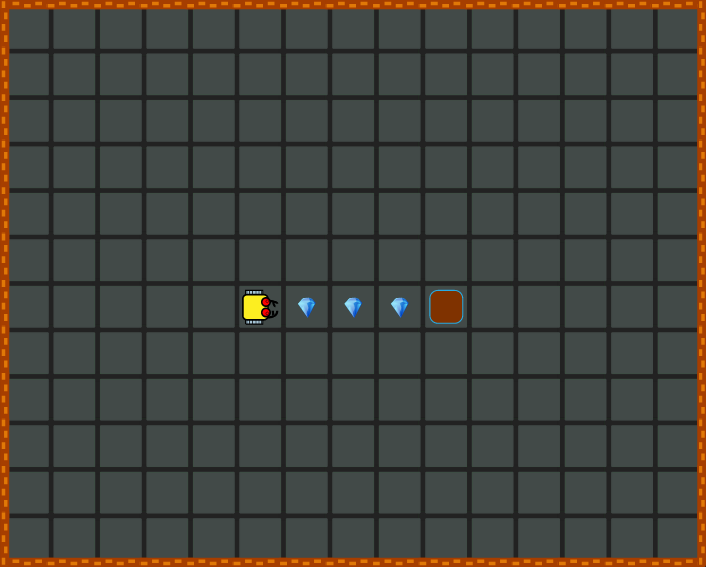
\includegraphics[height=0.4\textwidth]{imgk/b02.png}
\end{center}
\vspace{-4mm}
\caption{Collecting gems using the {\tt get} command.}
\label{fig:b02}
\vspace{-4mm}
\end{figure}
\noindent

\subsubsection{Solution}
\begin{verbatim}
go
get
go
get
go
get 
go
\end{verbatim}

\newpage
\subsection{}

{\em Write a program for Karel to collect the gem and return home! 

\begin{figure}[!ht]
\begin{center}
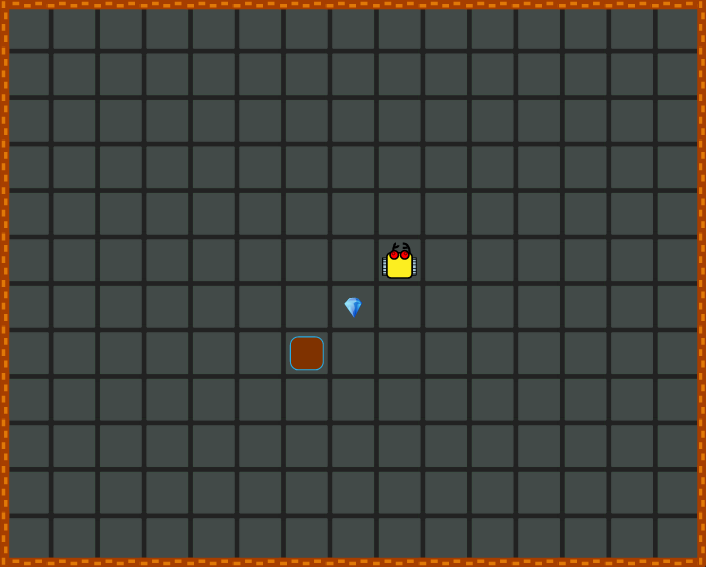
\includegraphics[height=0.4\textwidth]{imgk/b03.png}
\end{center}
\vspace{-4mm}
\caption{Turning to the left and to the right via the {\tt left} and {\tt right} commands.}
\label{fig:b03}
\vspace{-4mm}
\end{figure}
\noindent

\subsubsection{Solution}
\begin{verbatim}
left
go
left
go
get
right
go
left
go
\end{verbatim}

\newpage
\subsection{}

{\em Write a program for Karel to relocate the gem to the opposite 
end of the cross and return home!}



\begin{figure}[!ht]
\begin{center}
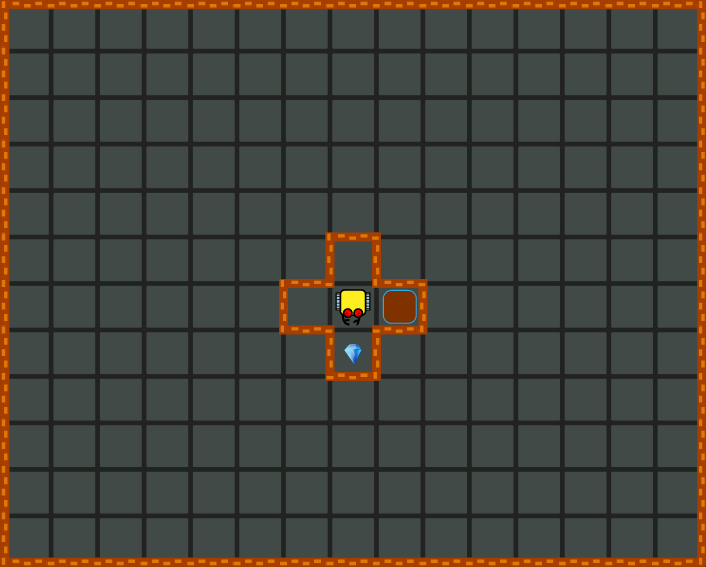
\includegraphics[height=0.4\textwidth]{imgk/b04.png}
\end{center}
\vspace{-4mm}
\caption{Relocating a gem requires both {\tt get} and {\tt put} commands.}
\label{fig:b04}
\vspace{-4mm}
\end{figure}
\noindent

\subsubsection{Solution}
\begin{verbatim}
go
get
left
left
go
go
put
left
left
go
left 
go
\end{verbatim}



\newpage
\setcounter{section}{5}
\section{Counting Loop}

\subsection{}

{\em Karel's home is ten steps away, so you could type {\tt go} ten times to get him home. However, using the {\tt repeat} command you can do this with only {\bf two lines}! 

\begin{figure}[!ht]
\begin{center}
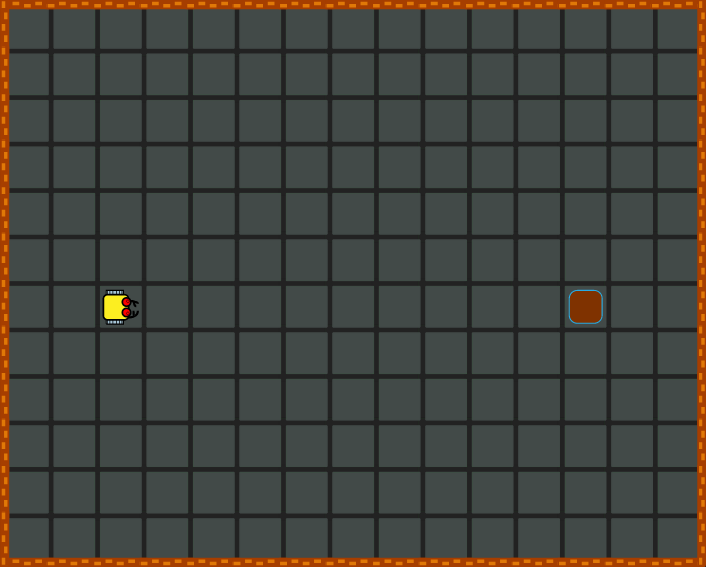
\includegraphics[height=0.4\textwidth]{imgk/c01.png}
\end{center}
\vspace{-4mm}
\caption{Karel gets home elegantly, using the {\tt repeat} command.}
\label{fig:c01}
\vspace{-4mm}
\end{figure}
\noindent

\subsubsection{Solution}
\begin{verbatim}
repeat 10
  go
\end{verbatim}

\newpage
\subsection{}

{\em Karel is about to find a pile of 12 gems! Write a program for the robot to collect the gems and get home. Use the {\tt repeat} command for any repeated action. 

\begin{figure}[!ht]
\begin{center}
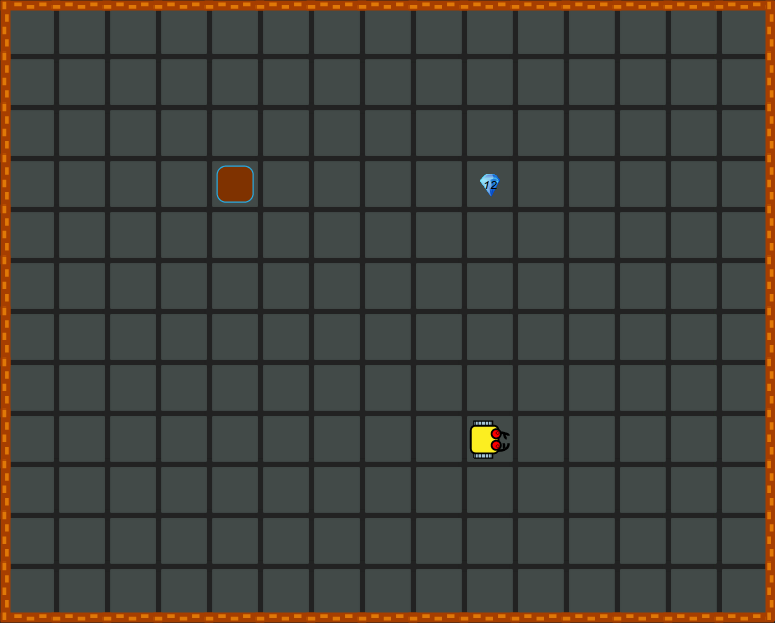
\includegraphics[height=0.4\textwidth]{imgk/c02.png}
\end{center}
\vspace{-4mm}
\caption{Karel is about to find a pile of 12 gems!}
\label{fig:c02}
\vspace{-10mm}
\end{figure}
\noindent

\subsubsection{Solution}
\begin{verbatim}
left
repeat 5
  go
repeat 12
  get
left
repeat 5
  go
\end{verbatim}

\newpage
\subsection{}

{\em Karel is feeling lucky today. He wants to just step outside his house, 
turn around five times, then pick up one gem somewhere, and get back inside!}


\begin{figure}[!ht]
\begin{center}
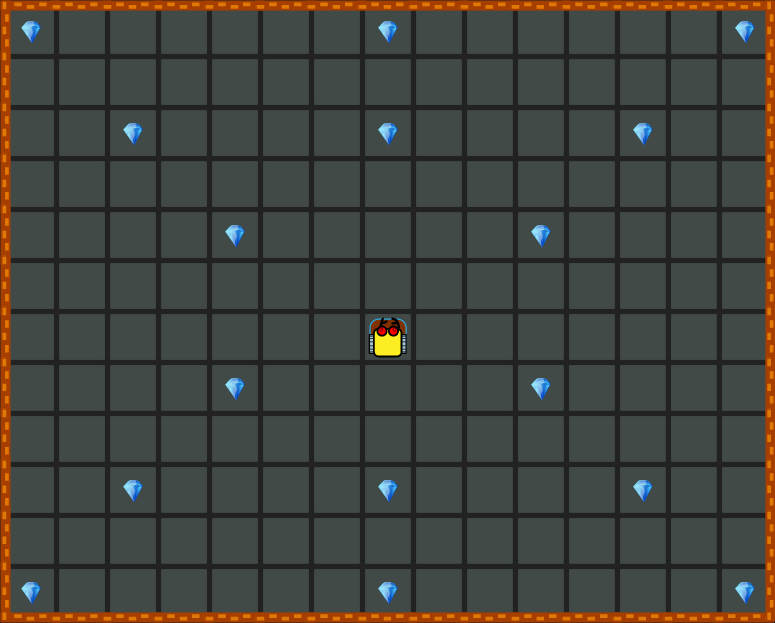
\includegraphics[height=0.4\textwidth]{imgk/c03.png}
\end{center}
\vspace{-4mm}
\caption{Karel is feeling lucky today.}
\label{fig:c03}
\vspace{-4mm}
\end{figure}
\noindent

\subsubsection{Solution}
\begin{verbatim}
go
repeat 20
  left
repeat 3 
  go
get
repeat 2
  left
repeat 4
  go
\end{verbatim}

\newpage
\subsection{}

{\em Karel needs to sell 10 of his oldest gems in order to make space for new ones. 
Write a program for the robot to step out of his garage, put 10 gems on the ground, 
and then turn back and get back inside! Use the {\tt repeat} command for any repeated 
action.}


\begin{figure}[!ht]
\begin{center}
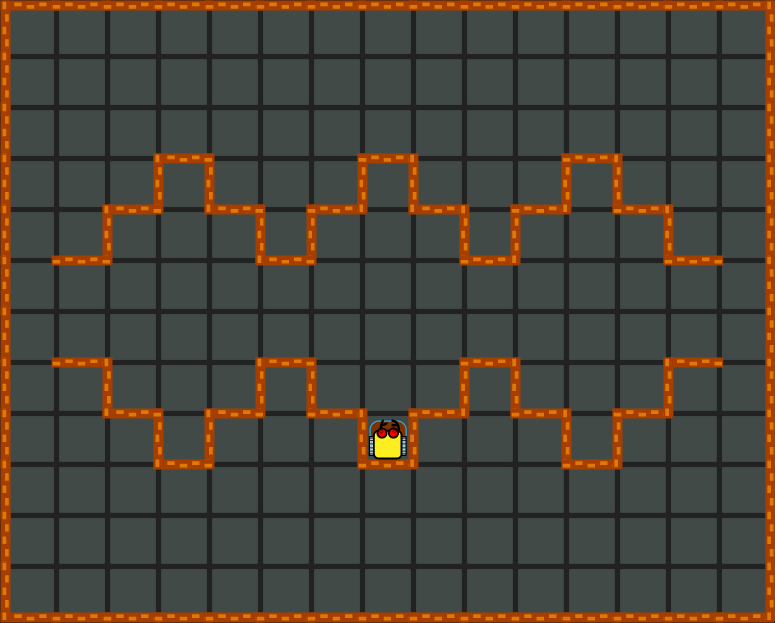
\includegraphics[height=0.4\textwidth]{imgk/c04.png}
\end{center}
\vspace{-4mm}
\caption{Karel is getting ready for garage sale.}
\label{fig:c04}
\vspace{-10mm}
\end{figure}
\noindent

\subsubsection{Solution}
\begin{verbatim}
go
repeat 10
  put
repeat 2
  left
go
\end{verbatim}


\newpage
\subsection{}

{\em Write a program for Karel to collect all nine gems and get home! 
Writing one command per line, your program should not have more 
than three lines.}.

\begin{figure}[!ht]
\begin{center}
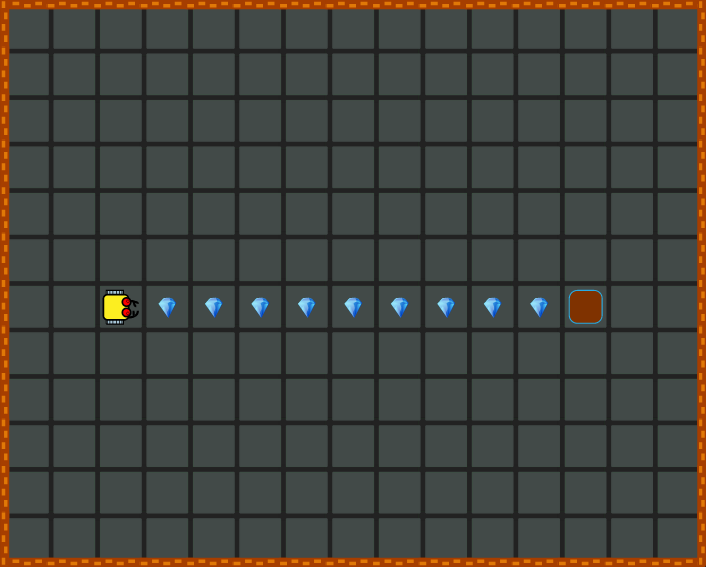
\includegraphics[height=0.4\textwidth]{imgk/c05.png}
\end{center}
\vspace{-4mm}
\caption{Nine gems are between Karel and his home.}
\label{fig:c05}
%\vspace{-10mm}
\end{figure}
\noindent

\subsubsection{Solution}
\begin{verbatim}
repeat 10
  go
  get
\end{verbatim}

%%%%%%%%%%%%%%%%%%%%%%%%%%%%%%%%%%%%%%%%%%%%%%%%%%%%%%%%%%%%%%%%%%%%%%%%%%%%%%%

\newpage
\iffullversion
\else
\vbox{}
\vfill
\pagestyle{empty}
    \begin{center}
    {\huge \color{red}END OF PREVIEW}\\[2cm]

\centerline{\Large Please consider:}
\vspace{1cm}

{\Large \bf Purchasing Online Course with Curriculum}
\vspace{1cm}

    {\Large or,}\\[1cm]

{\Large \bf Ordering Textbook}
\vspace{1cm}

    {\Large Visit {\tt http://introtoprogramming.net}. \\[2cm]
}
\end{center}
{\bf The course includes}:
\begin{itemize}
\item Access to full version of textbook and solution manual.
\item One-click download of interactive review question worksheets.
\item One-click download of interactive programming exercises.
\item One-click distribution to students in your class.
\item One-click collection, automated grading, and progress monitoring.
\item Access to all answers and solution programs.
\end{itemize}

\vfill
    \end{document}
\fi

\newpage
\setcounter{section}{7}
\section{Conditions}

\subsection{}

{\em Several gems lie on the ground between the robot and his home which is 10 steps away. 
He cannot see where the gems are though. 
Write a program for Karel to collect all gems and get home. With one command per 
line, your program should have at most 4 lines.}


\begin{figure}[!ht]
\begin{center}
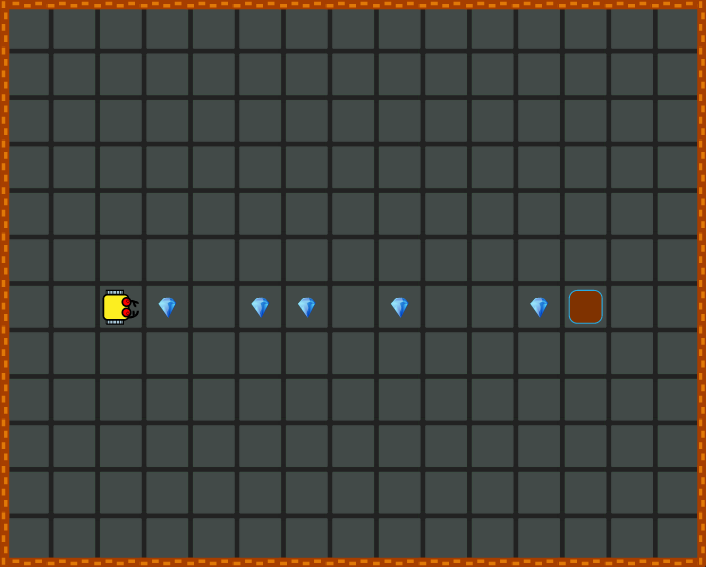
\includegraphics[height=0.4\textwidth]{imgk/d01.png}
\end{center}
\vspace{-4mm}
\caption{Several gems are at random positions between the robot and his home.}
\label{fig:d01}
\vspace{-4mm}
\end{figure}
\noindent

\subsubsection{Solution}
\begin{verbatim}
repeat 10
  if gem
    get
  go
\end{verbatim}

\newpage
\subsection{}

{\em Karel is walking on a meadows that is covered with irregularly 
scattered stones. Write a program for the robot to get to his home, 
avoiding stones, and collecting all gems!  }


\begin{figure}[!ht]
\begin{center}
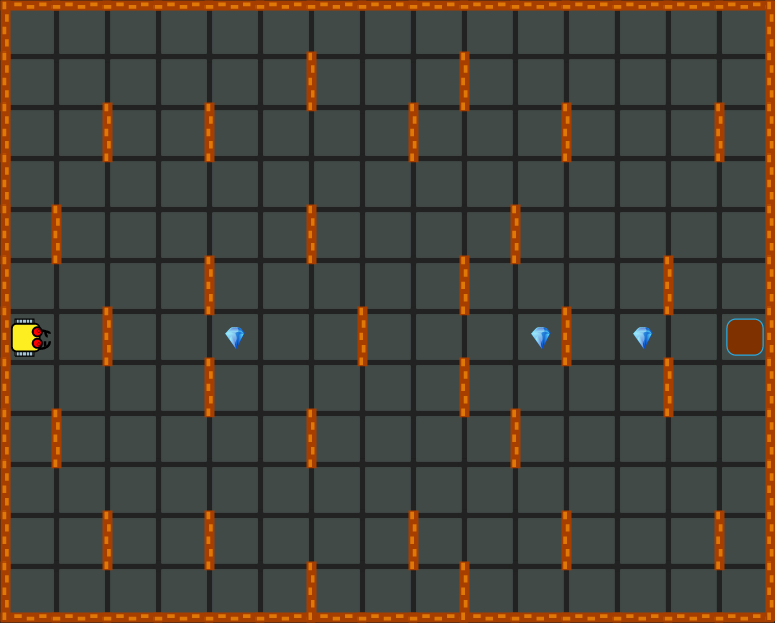
\includegraphics[height=0.4\textwidth]{imgk/d02.png}
\end{center}
\vspace{-4mm}
\caption{Karel is crossing a stony meadows.}
\label{fig:d02}
\vspace{-10mm}
\end{figure}
\noindent

\subsubsection{Solution}
\begin{verbatim}
repeat 14
  if gem
    get
  if not wall
    # you can go:
    go
  else
    # avoid the stone:
    left
    go
    repeat 2
      right
      go
    left
\end{verbatim}

\newpage
\subsection{}

{\em Karel stores all his gems in a secret chest in his cellar. 
Currently, some shelves are empty. Write a program for Karel to 
inspect all shelves and put a gem where one is missing! After that, he needs to get 
home as usual. With one 
command per line, your program should have at most 7 lines.}

\begin{figure}[!ht]
\begin{center}
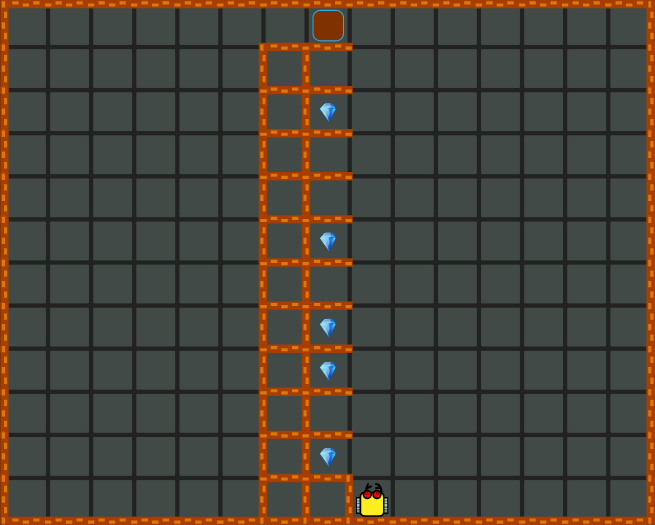
\includegraphics[height=0.4\textwidth]{imgk/d03.png}
\end{center}
\vspace{-4mm}
\caption{Filling empty shelves with gems.}
\label{fig:d03}
\vspace{-4mm}
\end{figure}
\noindent


\subsubsection{Solution}
\begin{verbatim}
repeat 11
  go
  left
  go
  if not gem
    put
  repeat 2
    left
  go
  left
\end{verbatim}

\newpage
\section{Conditional Loop}

\subsection{}

{\em Karel is somewhere in the maze, facing a random direction. Write a program for the robot to get 
to his home which is in the south-west corner!}

\begin{figure}[!ht]
\begin{center}
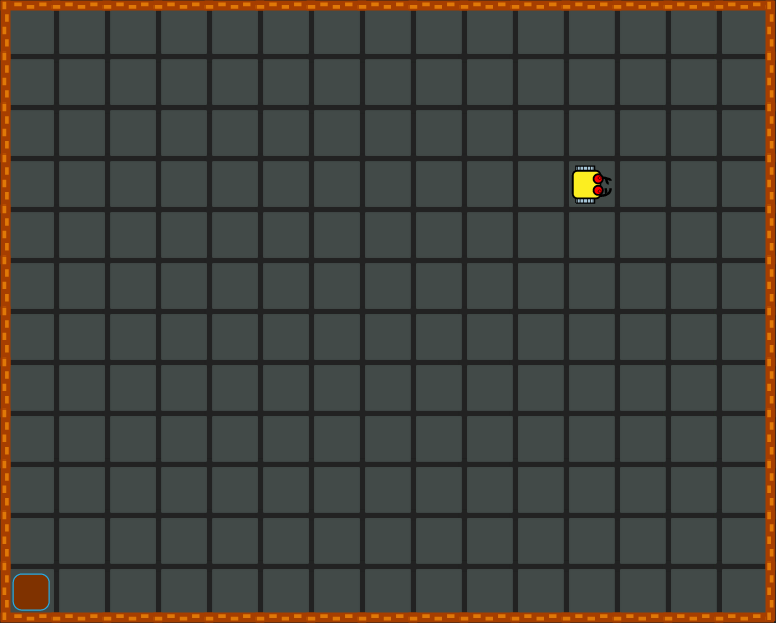
\includegraphics[height=0.4\textwidth]{imgk/e01.png}
\end{center}
\vspace{-4mm}
\caption{Karel only knows that his home is in the SW corner of the maze.}
\label{fig:e01}
\end{figure}
\noindent

\subsubsection{Solution}
\begin{verbatim}
# orient the robot to face north:
while not north
  left
# now turn him to face south:
repeat 2
  left
# go to the south border of maze:
while not wall
  go
# turn right:
right
# walk straight home:
while not home
  go
\end{verbatim}


\newpage
\subsection{}

{\em Karel's friends are hiding. To find them, he has to straight ahead 
and whenever he finds a gem, he has to collect it, 
turn left, and keep walking. Eventually, they said, he will get to the place 
where they are. Write a program for Karel to find his friends!}


\begin{figure}[!ht]
\begin{center}
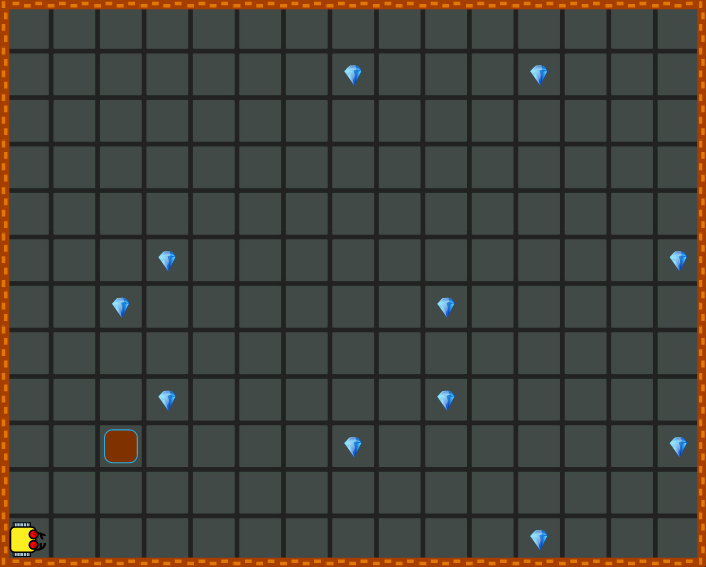
\includegraphics[height=0.4\textwidth]{imgk/e02.png}
\end{center}
\vspace{-4mm}
\caption{Karel plays hide-and-seek with his friends.}
\label{fig:e02}
\end{figure}
\noindent

\subsubsection{Solution}
\begin{verbatim}
while not home
  if not wall
    go
  if gem
    left
    get
\end{verbatim}

\newpage
\subsection{}

{\em Karel stands next to a straight wall and he knows that his home is somewhere on the other side of it. He does not know how long the wall is, nor the exact position of his home. Write a program for the robot to get there!}

\begin{figure}[!ht]
\begin{center}
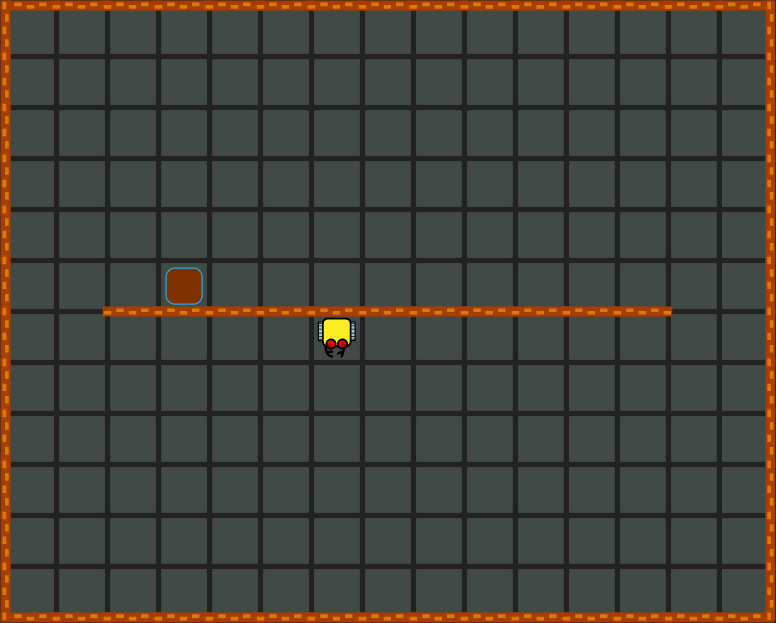
\includegraphics[height=0.4\textwidth]{imgk/e03.png}
\end{center}
\vspace{-4mm}
\caption{Karel only knows that his home is on the other side of the wall.}
\label{fig:e03}
\end{figure}
\noindent

\subsubsection{Solution}
\begin{verbatim}
# align the robot with the wall:
while not wall
  left
right

while not home
  go
  left
  if not wall
    # we are at the end
    go
    left
  else
    # not the end yet
    right
\end{verbatim}

\newpage
\section{Custom Commands}

\subsection{}

{\em This time Karel has to collect all four stars of gems!}

\begin{figure}[!ht]
\begin{center}
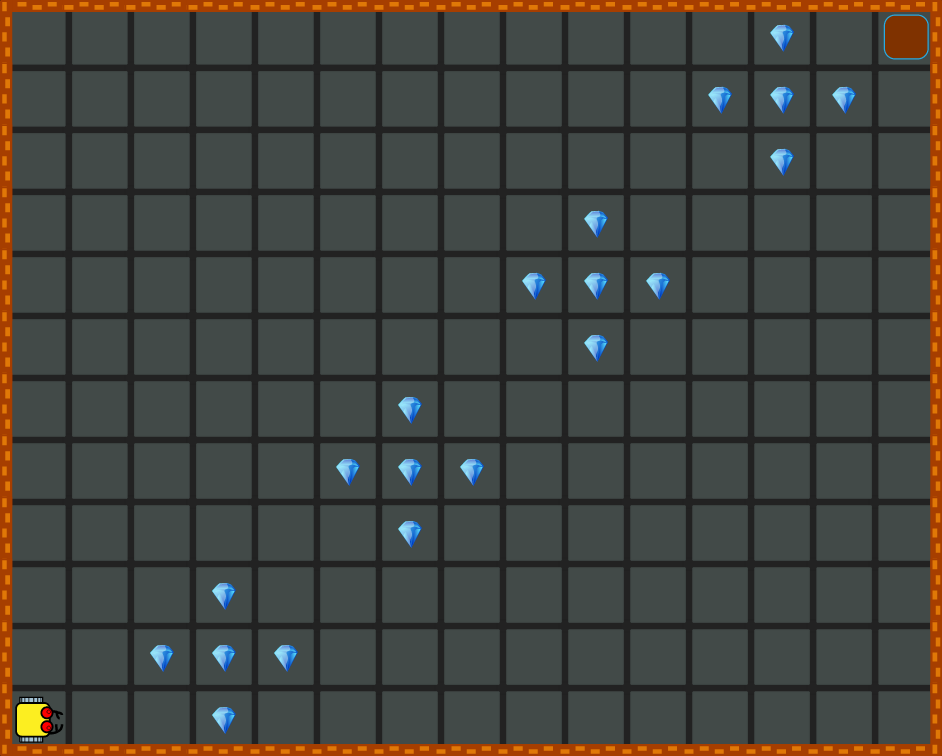
\includegraphics[height=0.4\textwidth]{imgk/f01.png}
\end{center}
\vspace{-4mm}
\caption{Karel needs to collect four stars of gems.}
\label{fig:f01}
\end{figure}
\noindent

\subsubsection{Solution}
\begin{verbatim}
# Shortcut for three commands:
def gogetgo
  go
  get
  go

# PIck one star:
def getstar
  repeat 2
    go
  repeat 4
    gogetgo
    left
  go
  left
  gogetgo

# Main program:
repeat 3
  getstar
  go
  right
getstar
right
repeat 3
  go
\end{verbatim}


\newpage
\subsection{}

{\em Write a program for the robot to move the 6x6 square of gems to the 
opposite corner of the maze. The task is finished when the robot is back home.}

\begin{figure}[!ht]
\begin{center}
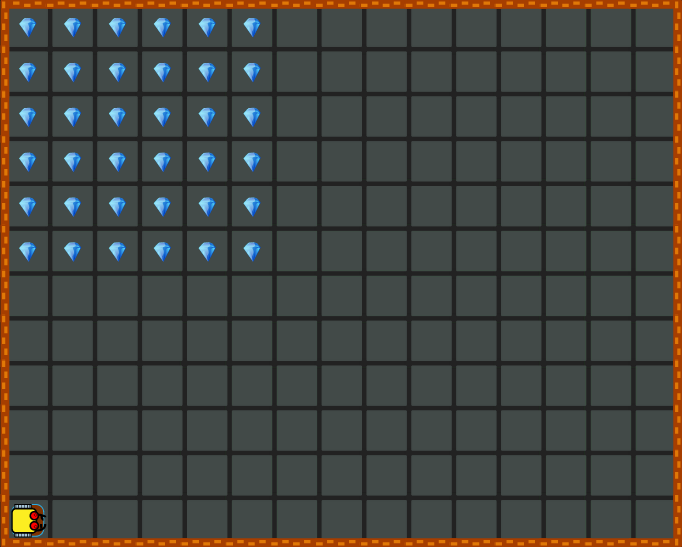
\includegraphics[height=0.4\textwidth]{imgk/f02.png}
\end{center}
\vspace{-4mm}
\caption{Karel needs to move the gems to the opposite corner of the maze.}
\label{fig:f02}
\end{figure}
\noindent

\subsubsection{Solution}
\begin{verbatim}
# Define function to either
# get or put a gem:
def try
  if gem
    get
  else
    if not empty
      put

# Do this for one column:
def column
  repeat 5
    try 
    go
  try
      
# Define function to 
# traverse the square:
def traverse
  repeat 3
    column
    right
    go
    right
    column
    left
    # Only used for the 
    # putting part:
    if not wall
      go 
      left

# Get there:
left
repeat 6
  go
   
# Collect gems:
traverse

# Move to the lower 
# left corner:
repeat 2
  left
while not wall
  go
left
repeat 3
  go
left

# Put the gems:
traverse

# Get homw:
repeat 2
  left
while not home
  go
\end{verbatim}

\newpage

\subsection{}

{\em Write a program for Karel to search all cells and collect all eggs (gems) that he can find. The task is finished when the robot is back home.}


\begin{figure}[!ht]
\begin{center}
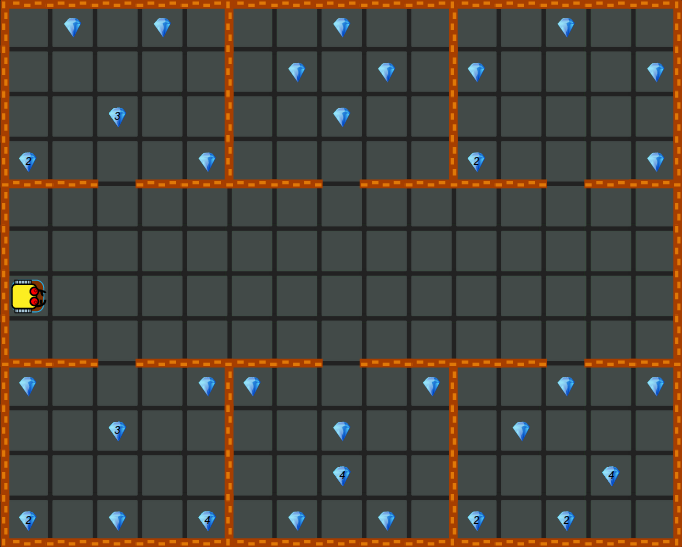
\includegraphics[height=0.4\textwidth]{imgk/f03.png}
\end{center}
\vspace{-4mm}
\caption{Easter is here, Karel is on egg hunt!}
\label{fig:f03}
\end{figure}
\noindent

\subsubsection{Solution}
\begin{verbatim}
# Get all gems in pile:
def getall
  while gem
    get

# Move forward one step
# and get gem if any:
def move
  go
  getall
    
# Move 2 times:
def move2
  repeat 2
    move
    
# Move 3 times:
def move3
  repeat 3
    move

# Move 4 times:
def move4
  repeat 4
    move

# Search one cell (assumes
# that Karel stands in front
# of the entrance):
def onecell
  move
  right
  move2
  left
  move3
  left
  move4
  left
  move3
  left
  move
  left
  move2
  right
  move2
  right
  move
  right
  move
  left
  move2

# Go to the next cell:
def gotonext
  left
  repeat 5
    go
  left
  
# Search three cells:
def searchthree
  repeat 2
    onecell
    gotonext
  onecell
  
# Go to the first cell:
move2
left
move2

# Search top cells:
searchthree

# Move across:
move3

# Search bottom cells:
searchthree

# Return home:
go
left
repeat 2
  go
\end{verbatim}

\newpage
\subsection{}

{\em Karel is a blind carpenter who needs to install windows (gems) into a newly built house. All he knows is that the house is a rectangle and that each window is exactly one tile large, But he can't see where the openings for the windows are. Install the windows and return home!}


\begin{figure}[!ht]
\begin{center}
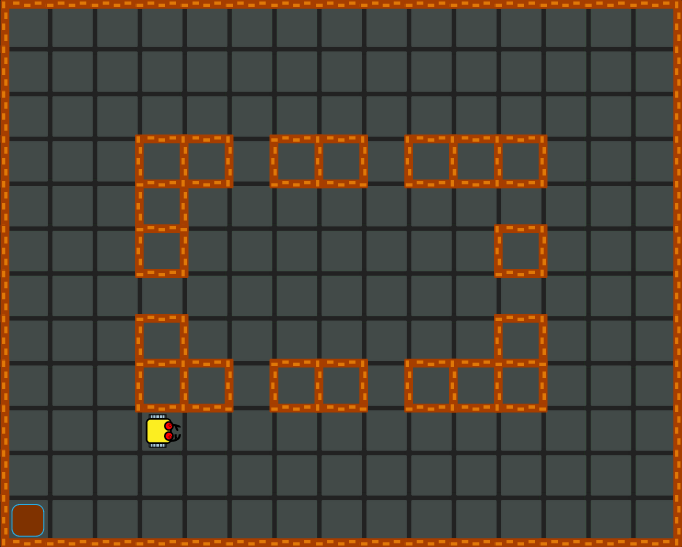
\includegraphics[height=0.4\textwidth]{imgk/f04.png}
\end{center}
\vspace{-4mm}
\caption{This time Karel installs windows.}
\label{fig:f04}
\end{figure}
\noindent

\subsubsection{Solution}
\begin{verbatim}
# Find nearest corner:
def find_corner
  left
  while wall
    right
    if not home
      go
      left
    
# Find out whether the opening
# in front of you is a window
# slot of the corner of the house. 
def check_window
  if not home
    go
    right
    if wall
      put
      right
      go
      left
      go
    else
      left
    
# Main program:
while not home
  find_corner
  check_window
\end{verbatim}

\newpage
\subsection{}

{\em Karel is on a pirate ship! Write a program for him to collect all 
gems and run away (to his home) before the pirates are back. Here Karel 
needs to be extremely efficient to survive. Therefore, there should be 
no repeating parts whatsoever in your program!}


\begin{figure}[!ht]
\begin{center}
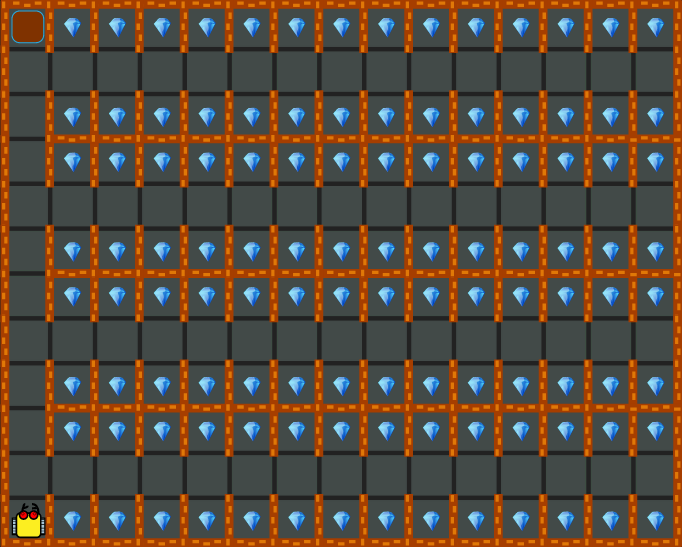
\includegraphics[height=0.4\textwidth]{imgk/f05.png}
\end{center}
\vspace{-4mm}
\caption{Karel found a pirate treasure.}
\label{fig:f05}
\end{figure}
\noindent

\subsubsection{Solution}
\begin{verbatim}
# The three commands below are 
# elementary and you should be
# defining them as the last thing.
# Read this code from below. 
# Long step.
def longstep
  repeat 2
    go

# Version of longstep where Karel
# may get home.
def longstephome
  go
  if not home 
    go
    
# Turn back.
def turnback
  repeat 2
    left

# Get pair of gems that lie across 
# the aisle, and move to next pair.
# This should be your third part
# of code to write.
def gettwo
  go
  left
  go
  get
  turnback
  longstep
  get
  turnback
  go
  right

# Empty an entire aisle and 
# get ready for the next one.
# This should be your second 
# part of the code to write.
def emptyaisle
  go
  right
  while not wall
    gettwo
  turnback
  while not wall
    go
  right
  longstephome
    
# Karel does not know how many 
# aisles there are, so he will 
# be emptying them until he 
# gets home. This should be your
# first part of code to write.
while not home
  emptyaisle
\end{verbatim}

\newpage
\subsection{}

{\em Write a program for Karel to climb the staircase, collect all gems, and 
get home. The number of steps in the staircase is random. }


\begin{figure}[!ht]
\begin{center}
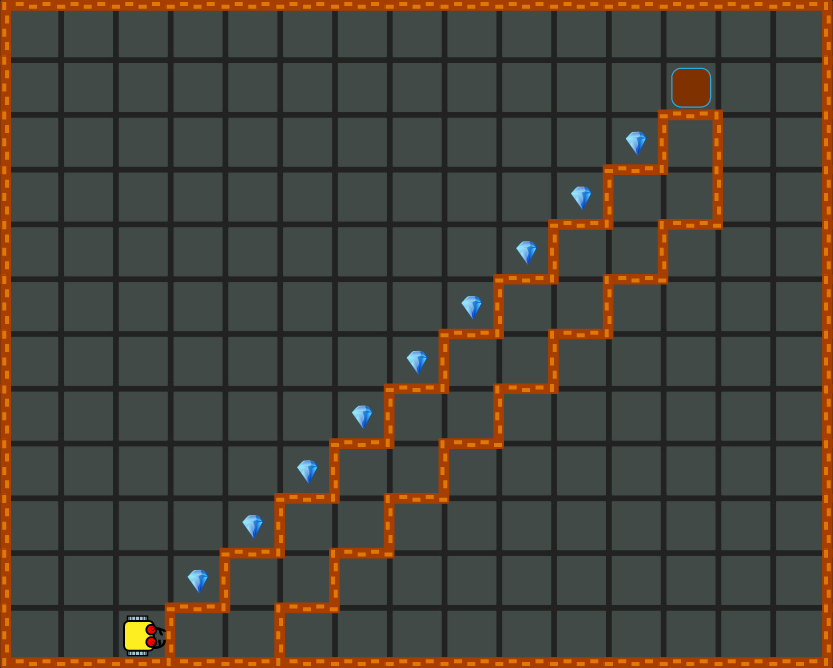
\includegraphics[height=0.4\textwidth]{imgk/f06.png}
\end{center}
\vspace{-4mm}
\caption{This time Karel has to do some climbing.}
\label{fig:f06}
\end{figure}
\noindent

\subsubsection{Solution}
\begin{verbatim}
def onestep
  left
  go
  right
  go 
  get
  
while not home
  onestep
\end{verbatim}

\newpage
\subsection{}

{\em Write a program for Karel to pluck all flowers that grow at the fence of his garden (gems), and get back home! Note two levels of repetition.}


\begin{figure}[!ht]
\begin{center}
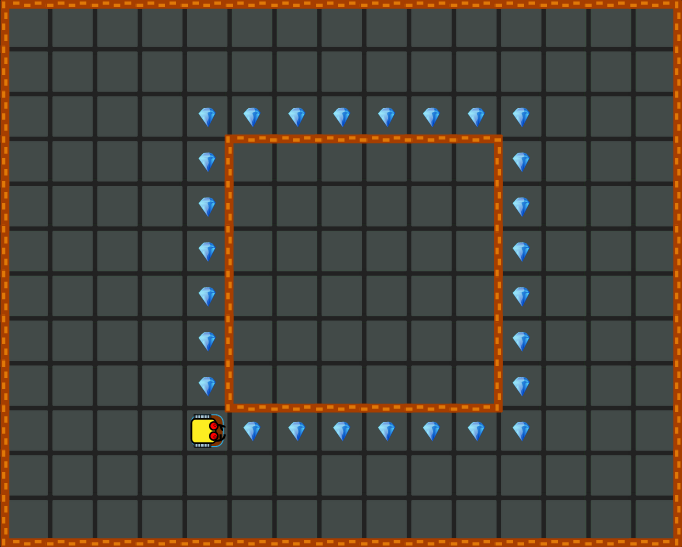
\includegraphics[height=0.4\textwidth]{imgk/f07.png}
\end{center}
\vspace{-4mm}
\caption{Karel is plucking flowers along his fence.}
\label{fig:f07}
\end{figure}
\noindent

\subsubsection{Solution}
\begin{verbatim}
repeat 4
  repeat 7
    go
    get
  left
\end{verbatim}

\newpage
\subsection{}

{\em Karel has three gems in his bag, that he wants to give to his three friends R2, D2 and Marvin who live close by. Write a program for Karel to put a gem on the ground in the middle of each friend's home, and then return to his own home.}


\begin{figure}[!ht]
\begin{center}
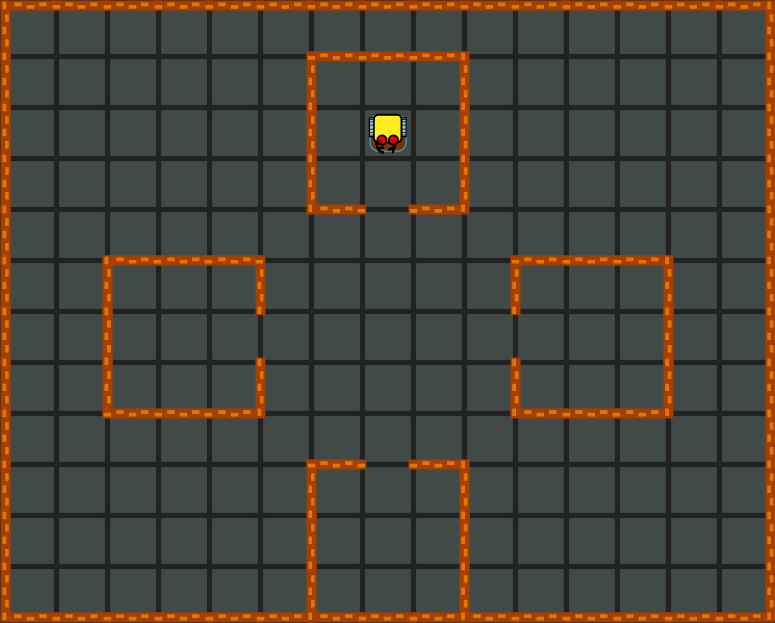
\includegraphics[height=0.4\textwidth]{imgk/f08.png}
\end{center}
\vspace{-4mm}
\caption{Karel is going to give gems to his three friends R2, D2 and Marvin.}
\label{fig:f08}
\end{figure}
\noindent

\subsubsection{Solution}
\begin{verbatim}
# go four steps forward:
def foursteps
  repeat 4
    go

repeat 4
  # go to the middle:
  foursteps
  # turn to the left:
  left
  # enter friend's house:
  foursteps
  # put a gem on the ground:
  put
  # turn back:
  repeat 2
    left
\end{verbatim}

\newpage
\subsection{}

{\em Karel stands in front of a diamond rectangle of unknown dimensions. Write a program for the robot to walk around the rectangle, collect all gems, and get home!}


\begin{figure}[!ht]
\begin{center}
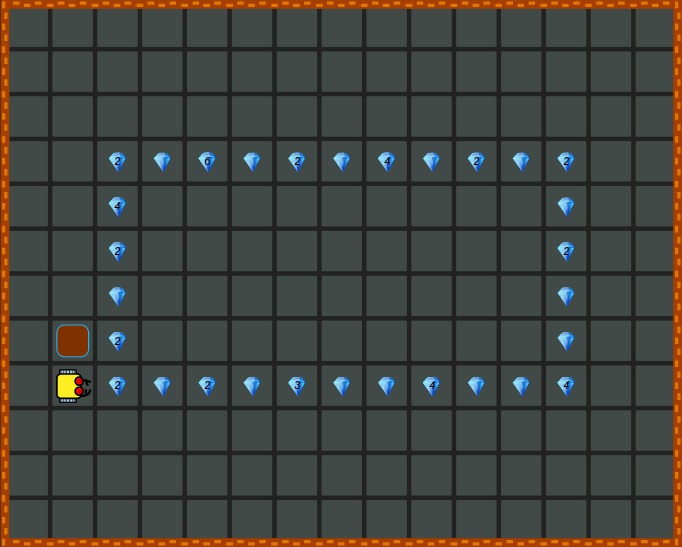
\includegraphics[height=0.4\textwidth]{imgk/f09.png}
\end{center}
\vspace{-4mm}
\caption{This time Karel does not know the size of the rectangle.}
\label{fig:f09}
\end{figure}
\noindent

\subsubsection{Solution}
\begin{verbatim}
go
while not home
  while gem
    # collect all gems in the pile:
    while gem
      get
    # move on one step:
    go
  # we reached the end - turn 
  # only if not home yet:
  if not home
    repeat 2
      left
    go
    right
    go
\end{verbatim}

\newpage
\subsection{}

{\em In this maze, gems are distributed randomly along the walls. Otherwise 
the maze is empty. Karel's home is in the south-west corner, and the robot 
stands on the right of it, facing east. Write a program for Karel to collect 
all the gems and return home!}

\begin{figure}[!ht]
\begin{center}
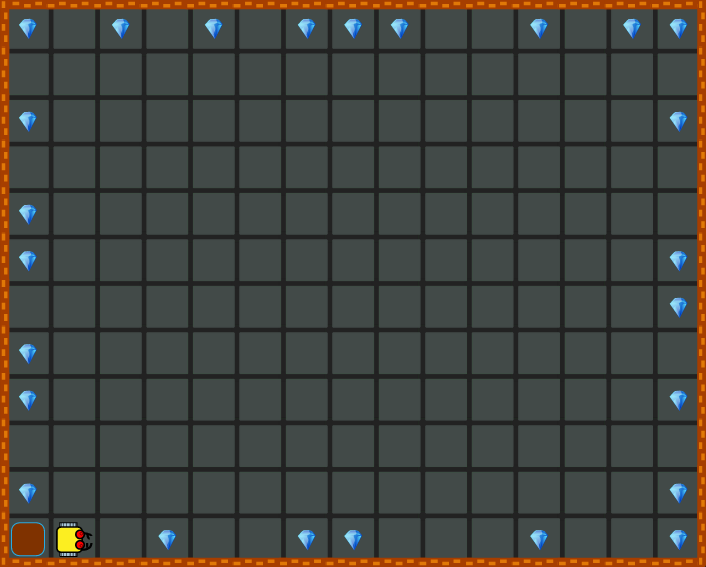
\includegraphics[height=0.4\textwidth]{imgk/f10.png}
\end{center}
\vspace{-4mm}
\caption{Gem Jam!}
\label{fig:f10}
\end{figure}
\noindent

\subsubsection{Solution}
\begin{verbatim}
while not home
  while not wall
    if gem
      get
    go
  left
\end{verbatim}

\newpage
\subsection{}

{\em Write a program for Karel to collect all gems and enter his home!}

\begin{figure}[!ht]
\begin{center}
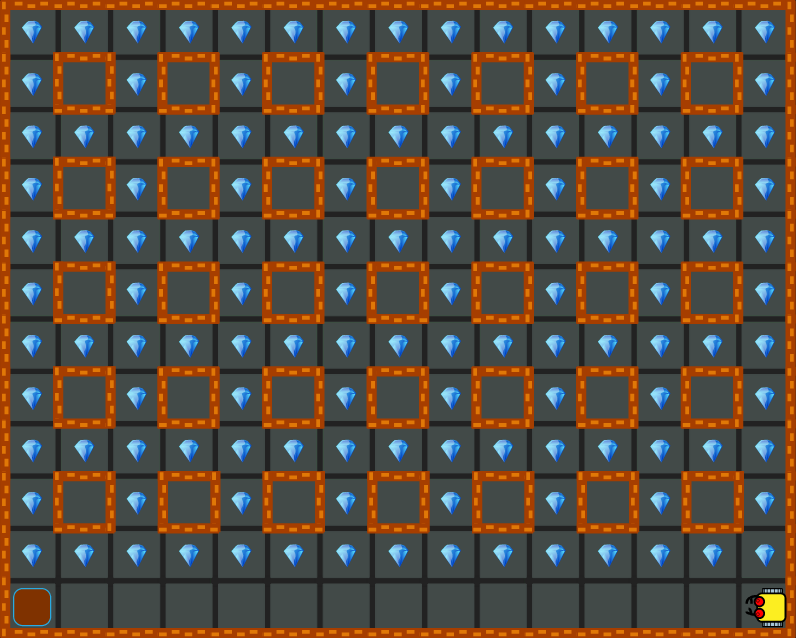
\includegraphics[height=0.4\textwidth]{imgk/f11.png}
\end{center}
\vspace{-4mm}
\caption{The Matrix.}
\label{fig:f11}
\end{figure}
\noindent

\subsubsection{Solution}
\begin{verbatim}
# Pick up 15 gems:
def get15
  if gem
    get
  repeat 14
    go
    if gem
      get
      
# Pick up 11 gems:
def get11
  if gem
    get
  repeat 10
    go
    if gem
      get
      
# Left turn:
def leftturn
  left
  go
  if gem 
    get
  go
  left
  
# Right turn:
def rightturn
  right
  go
  if gem 
    get
  go
  right

# Clear two columns:
def clear2columns
  get11
  leftturn
  get11
  rightturn

# Clear two rows:
def clear2rows
  get15
  leftturn
  get15
  rightturn
  
# Get to initial position:     
right
go

# First clear all vertical aisles:
repeat 3
  clear2columns
get11
leftturn
get11

# Get in position to clear horizontal
# aisles:
left

# Clear all horizontal aisles:
repeat 2
  clear2rows
get15
leftturn
get15

# Get ready to return home:
left

# Go home:
while not home
  go
\end{verbatim}

\newpage
\subsection{}

{\em Karel is escaping from the Alcatraz prison! At the moment he is in an underground labyrinth with many random tunnels but only one of them leads to his freedom. Use the right-hand rule to find your way out!}


\begin{figure}[!ht]
\begin{center}
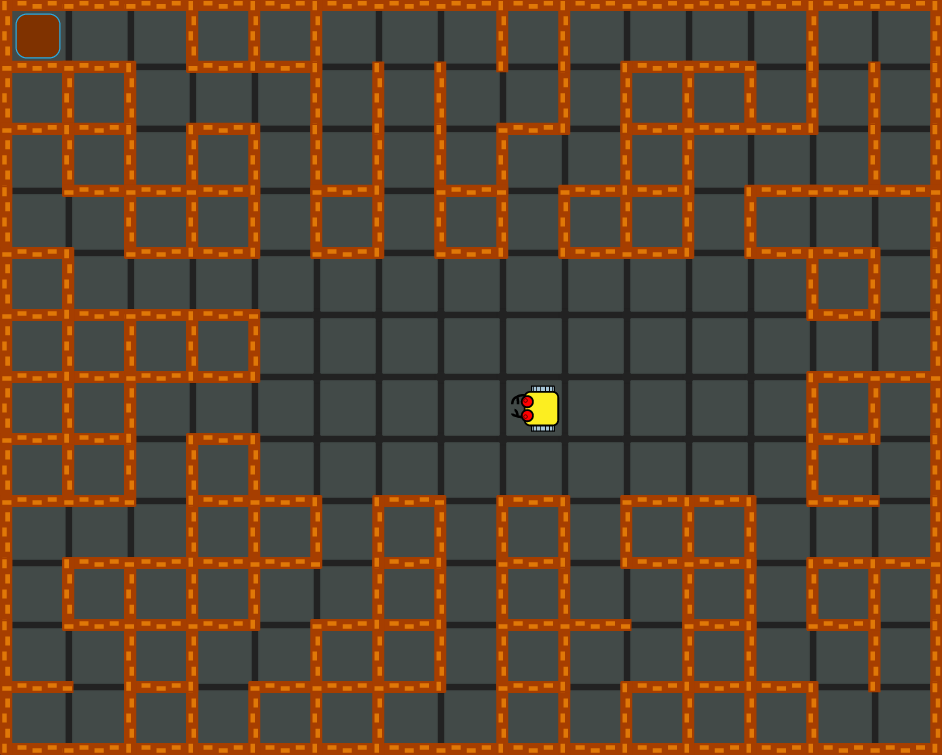
\includegraphics[height=0.4\textwidth]{imgk/f12.png}
\end{center}
\vspace{-4mm}
\caption{Karel is escaping from the Alcatraz prison.}
\label{fig:f12}
\end{figure}
\noindent

\subsubsection{Solution}
\begin{verbatim}
# Align the robot so that wall is 
# on its right.
def align_with_wall
  while not wall 
    left
  left

# Make a step along the wall (and 
# around a corner if needed). Assumes 
# that wall is on your right. 
def step_along_wall
  while wall 
    left
  go
  # Check whether there is a corner.
  right
  if wall 
    left   # No corner.   
  else     # Corner.
    go
    right
    if wall 
      left
    else 
      go
      
# Step along the wall until you reach 
# home. Assumes that Karel stands next 
# to a wall that is connected to an 
# exterior wall.
def search_tunnels
  align_with_wall
  while not home
    step_along_wall

while not wall
  go
search_tunnels
\end{verbatim}

\newpage
\subsection{}

{\em Write a program for Karel to check the perimeter of the maze using the 
right-hand rule. Do not forget to pick up all gems that you find on the way.}

\begin{figure}[!ht]
\begin{center}
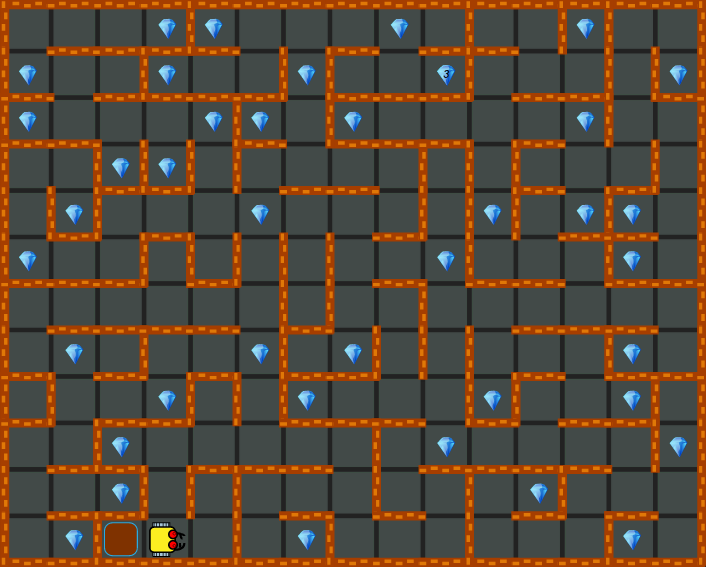
\includegraphics[height=0.4\textwidth]{imgk/f13.png}
\end{center}
\vspace{-4mm}
\caption{Border Patrol.}
\label{fig:f13}
\end{figure}
\noindent

\subsubsection{Solution}
\begin{verbatim}
# Align the robot so that wall is 
# on its right.
def align_with_wall
  while not wall 
    left
  left

# Make a step along the wall (and 
# around a corner if needed). Assumes 
# that wall is on your right. 
def step_along_wall
  while wall 
    left
  go
  if gem 
    get
  # Check whether there is a corner.
  right
  if wall 
    left   # No corner.   
  else     # Corner.
    go
    if gem 
      get
    right
    if wall 
      left
    else 
      go
      if gem 
        get

# Step along the wall until you reach 
# home. Assumes that Karel stands next 
# to a wall that is connected to an 
# exterior wall.
def border_patrol
  align_with_wall
  while not home
    step_along_wall

border_patrol
\end{verbatim}

\newpage
\subsection{}

{\em In an ancient Greek legend, princess Ariadne saved the life of her 
beloved Theseus by giving him a thread that he used to avoid getting lost 
in the maze of king Minos and kill a feared beast Minotaurus. Karel uses 
a similar technique - he leaves behind him a chain of gems that helps him 
to safely find his way back home. Your program needs to work for an 
arbitrary maze. You can assume that the string of gems is continuous 
and that it does not contain any loops.}

\begin{figure}[!ht]
\begin{center}
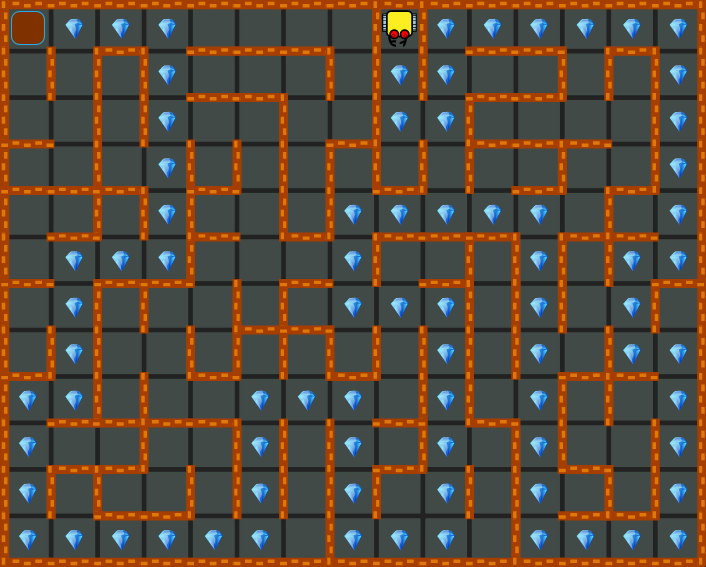
\includegraphics[height=0.4\textwidth]{imgk/f14.png}
\end{center}
\vspace{-4mm}
\caption{Maze of king Minos, home of the beast Minotaurus.}
\label{fig:f14}
\end{figure}
\noindent

\subsubsection{Solution}
\begin{verbatim}
# Turn back:
def back
  repeat 2
    left

# Program assumes that Karel faces the last gem.
# The chain of gems should not have loops.
def get_next_gem
  if not wall
    if not home
      go
      if gem 
        get
      else
        if not home
          back
          go
          left
          if not wall
            if not home
              go
              if gem 
                get
              else
                if not home
                  back
                  repeat 2 
                    go
                  get
          else
            if not home
              back
              go
              get
  else 
    left
    if not wall
      if not home
        go
        if gem 
          get
        else
          if not home
            back
            repeat 2 
              go
            get
    else
      if not home
        back
        go
        get

def ariadnes_thread
  while not home
    get_next_gem
        
ariadnes_thread
\end{verbatim}

\newpage
\section{Recursion}

\subsection{}

{\em Karel's favorite way to eat cheese is to peel one edge at a time. His brick of 
cheese is represented by a rectangle of gems. The rectangle has random dimensions
and the robot's initial position is at one of the corners, as shown in Fig. \ref{fig:g01}.
Write a recursive algorithm for the robot to eat all the cheese and return home!
 }
\begin{figure}[!ht]
\begin{center}
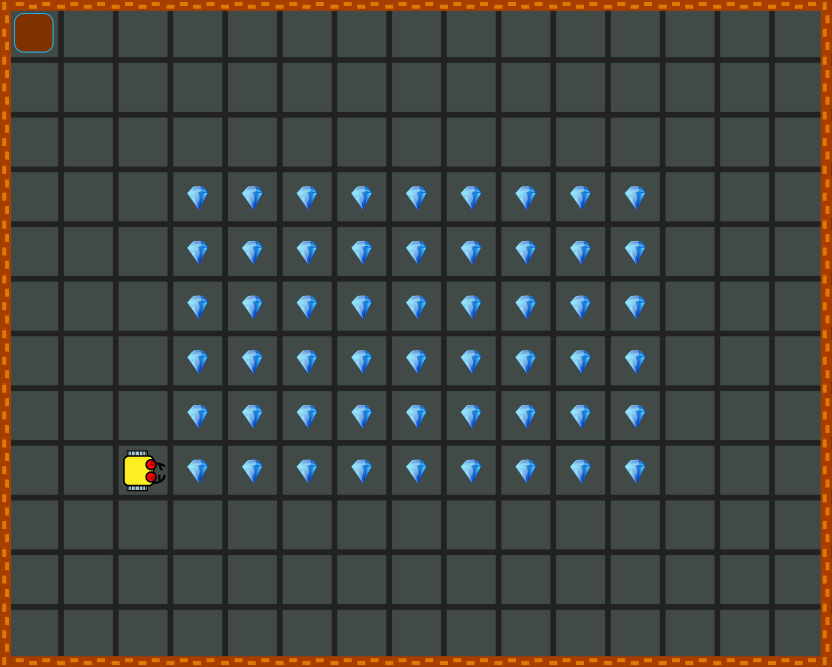
\includegraphics[height=0.4\textwidth]{imgk/g01.png}
\end{center}
\vspace{-4mm}
\caption{Karel is eating cheese.}
\label{fig:g01}
\end{figure}

\subsubsection{Solution}

\begin{verbatim}
def peel_edge
  go
  while gem
    get
    go
  repeat 3
    right
    go
  go
  if gem
    get
    peel_edge
      
# Eat the cheese:
peel_edge

# Return home:
while not north
  left
while not wall
go
left
while not home
  go
\end{verbatim}


\newpage
\subsection{}

{\em Karel stands at the entrance to a cave and wants to explore it. Write a recursive program for the robot to descend the staircase to the bottom, return back, and enter his home! The number of steps in the staircase is random.}
\begin{figure}[!ht]
\begin{center}
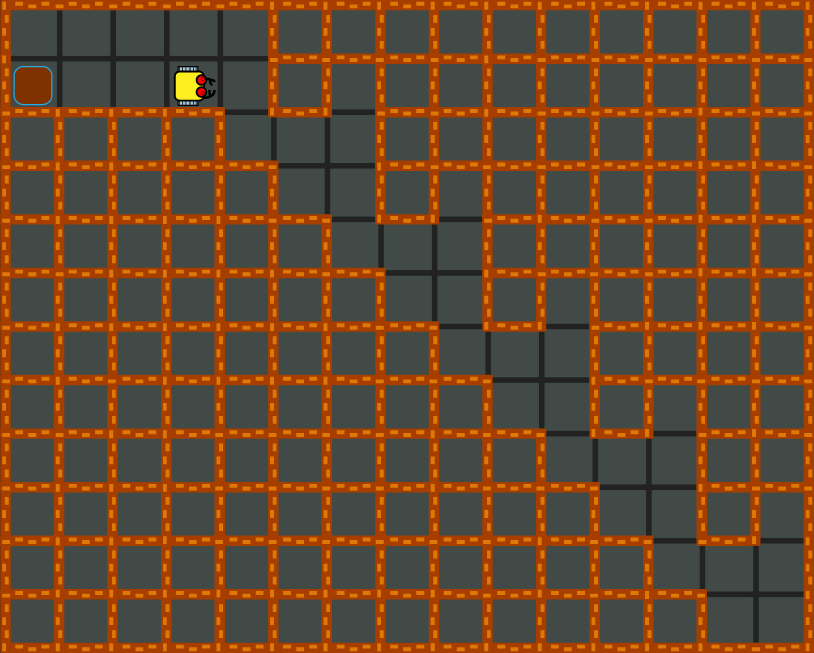
\includegraphics[height=0.4\textwidth]{imgk/g02.png}
\end{center}
\vspace{-4mm}
\caption{Karel became a speleologist.}
\label{fig:g02}
\end{figure}
\noindent


\subsubsection{Solution}

\begin{verbatim}
# Descend one step, explore the rest,
# and return:
def explore
  if not wall
    go
    right
    if not wall
      go
      left
      explore
      right
      go
      left
      go
    else
      right
      go
  else 
    repeat 2
      left
      go
    
# Explore cave and return home:
explore
while not home
  go
\end{verbatim}

\newpage
\subsection{}

{\em  Karel has many gems in his bag, and he needs to build a heap shown in Fig. \ref{fig:g03} before he can 
enter his home. Use recursion.}

\begin{figure}[!ht]
\begin{center}
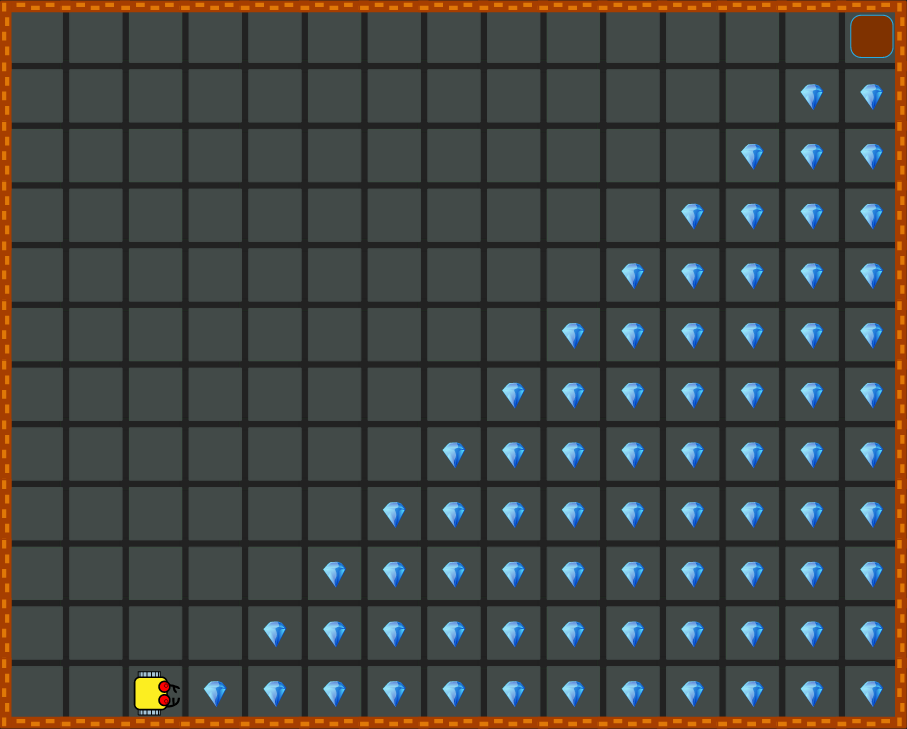
\includegraphics[height=0.4\textwidth]{imgk/g03.png}
\end{center}
\vspace{-4mm}
\caption{Karel needs to build a heap of gems before he can get home.}
\label{fig:g03}
\end{figure}

\subsubsection{Solution}

\begin{verbatim}
# Turn back.
def back
  repeat 2
    left
  
# Add layer of gems, return, and
# get ready for next layer.
def addlayer
  if not home
    while not wall 
      go
      put
    # Turn back and return.
    back
    while gem
      go
    back
    # Get ready for next layer.
    go
    left
    go 
    right
    addlayer
    
addlayer
\end{verbatim}

\newpage
\subsection{}

{\em Karel stands under a diamond tree, with his home next to him on the the right. 
The tree is random -- at any point it can have 
a branch in the north-west or in the north-east direction (or in both). Write a recursive 
algorithm for the robot to collect all gems from the tree and get home!  }

\begin{figure}[!ht]
\begin{center}
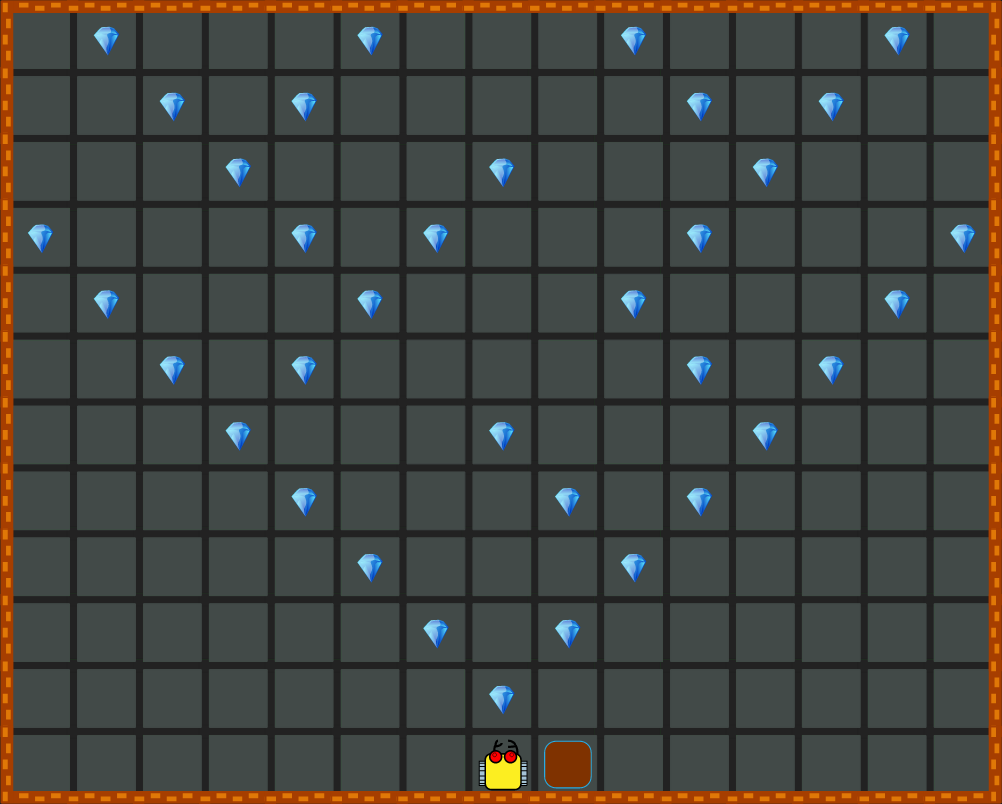
\includegraphics[height=0.4\textwidth]{imgk/g04.png}
\end{center}
\vspace{-4mm}
\caption{Karel is traversing a random diamond tree.}
\label{fig:g04}
\end{figure}
\noindent

\subsubsection{Solution}

\begin{verbatim}
# Turn back.
def back
  repeat 2
    left

# Right angle.
def rangle
  go
  right
  go
  
# Left angle.
def langle
  go
  left
  go
  
# Return from left branch to base.
def return_from_left_branch
  right
  rangle
  back
  
# Return from right branch to base.
def return_from_right_branch
  left
  langle
  back
  
# Robot faces left wall after 
# an attempt to find new branch 
# on the left.
def return_from_left_wall
  left
  go
  back
  
# Robot faces right wall after
# an attempt to find new branch 
# on the right.
def return_from_right_wall
  right
  go
  back
  
# Assumes that Karel stands on a gem.
def left_branch
  # Is there a wall in the North?
  if not wall
    go
    left
    # Is there a wall in the West?
    if not wall
      go
      right
      if gem
        climb_tree
      return_from_left_branch
    else
      return_from_left_wall

# Assumes that Karel stands on a gem.
def right_branch
  # Is there a wall in the North?
  if not wall
    go
    right
    # Is there a wall in the East?
    if not wall
      go
      left
      if gem
        climb_tree
      return_from_right_branch
    else
      return_from_right_wall

# Traverse recursively first the 
# left and then the right branch.
# Then pick up the base gem.
def climb_tree
  left_branch
  right_branch
  if gem
    get

# Move to tree.    
go
# Traverse it recursively.
climb_tree
# Go home.
right
rangle
\end{verbatim}

%%%%%%%%%%%%%%%%%%%%%%%%%%%%%%%%%%%%%%%%%%%%%%%%%%%%%%%%%%%%%%%%%%%%%%%%%%%%%%%%%%%
\newpage
\section{Variables}

\subsection{}

{\em Karel has an unknown number of gems in his bag. Write a function {\tt accounting} for the 
robot to count the gems and return their number. Then call the function and print the result.}

\begin{figure}[!ht]
\begin{center}
\includegraphics[height=0.4\textwidth]{imgk/h01.png}
\end{center}
\vspace{-4mm}
\caption{Karel is counting his gems.}
\label{fig:h01}
\end{figure}

\subsubsection{Solution}

\begin{verbatim}
def accounting
  num = zero
  while not empty
    put
    inc(num)
  return num

n = accounting
print "I have", n, "gems in the bag."
\end{verbatim}

\newpage
\subsection{}

{\em Karel stands inside of a room (rectangle) with unknown dimensions. Write function {\tt measure}  
where the robot will determine the width of the rectangle (in the west-east direction) and return it. 
Then call the function and print the result.}

\begin{figure}[!ht]
\begin{center}
\includegraphics[height=0.4\textwidth]{imgk/h02.png}
\end{center}
\vspace{-4mm}
\caption{Karel is measuring his room.}
\label{fig:h02}
\end{figure}
\noindent

\subsubsection{Solution}

\begin{verbatim}
def measure
  # Go to the west wall
  # and turn east:
  while not north
    left
  left
  while not wall
    go
  repeat 2
    left
  # Start measuring:
  len = zero
  while not wall
    inc(len)
    go
  return len
  
l = measure
print "Width of the room is", l
\end{verbatim}

\newpage
\subsection{}

{\em Write a function {\tt orchard} for the robot to count apples (gems) in his orchard. The position of 
trees as well as the number of apples per tree are random. The initial position of the robot is 
in the south-west corner, facing east. There are no walls
to crash into. After the function is ready, call it and print the result.}

\begin{figure}[!ht]
\begin{center}
\includegraphics[height=0.4\textwidth]{imgk/h03.png}
\end{center}
\vspace{-4mm}
\caption{Karel is counting apples in his orchard.}
\label{fig:h03}
\end{figure}
\noindent


\subsubsection{Solution}

\begin{verbatim}
def orchard
  num = zero
  repeat 6
    # Check the tile you stand on:
    while gem
      inc(num)
    # Check the rest of the row:
    while not wall
      go
      while gem
        inc(num)
    # Move to next row and turn back:
    left
    if not wall
      go
    left
    # Check the tile you stand on:
    while gem
      inc(num)
    # Check the rest of the row:
    while not wall
      go
      while gem
        inc(num)
    # Move to next row and turn back:
    right
    if not wall
      go
    right

n = orchard
print "There are", n, "apples in the orchard."
\end{verbatim}

\newpage
\subsection{}

{\em Karel needs new carpet! Write a function {\tt carpet} for the robot to calculate 
the area (number of tiles) of his apartment and return it. After that, call the function 
and print the result. His apartment is random but it has a simple shape -- wherever 
the robot stands, when he goes north, south, east or west he will always reach exterior wall.
The initial position of the robot is at the west wall of the bottom row, facing east.}

\begin{figure}[!ht]
\begin{center}
\includegraphics[height=0.4\textwidth]{imgk/h04.png}
\end{center}
\vspace{-4mm}
\caption{Karel is measuring area of his apartment before installing new carpet.}
\label{fig:h04}
\end{figure}
\noindent

\subsubsection{Solution}

\begin{verbatim}
# Count tiles in one row. Assumes
# that Karel stands at the West end 
# of the row, facing East: 
def check_row
  n = 1
  while not wall
    go 
    inc(n)
  return n
  
# Assumes that Karel is at the 
# East end of a row, facing East:
def one_row_up
  finished = False
  left
  while wall
    left
    if not wall 
      go
    else 
      finished = True 
    right
  go
  return finished

# Move to the West end of row 
# and turn East. Assumes that 
# Karel faces North:
def get_west
  left
  while not wall
    go
  repeat 2
    left
  
# Measure the area:
def carpet
  a = check_row
  while one_row_up
    get_west
    inc(a, check_row)
  return a
  
# Calculate and print apartment area:
area = carpet
print "Carpet size =", area
\end{verbatim}

\newpage
\section{Logic}

\subsection{}

{\em Each 3x5 box contains a random integer number between 0 and 9. Write a function "readnumber" 
where Karel enters a box, determines the number in it, and returns it. Initial position of the 
robot is at the entrance of the box, facing north. The final position of the robot should be the same. 
Use this function to determine the numbers in the three boxes as shown in the screenshot. }

\begin{figure}[!ht]
\begin{center}
\includegraphics[height=0.4\textwidth]{imgk/i01.png}
\end{center}
\vspace{-4mm}
\caption{Karel is learning to recognize numbers.}
\label{fig:g10}
\end{figure}
\noindent

\subsubsection{Solution}

\begin{verbatim}
# Make two steps:
def go2
  repeat 2 
    go

# Read number in box:
def readnumber
  # First detect gems
  # at key positions:
  go
  gem10 = gem
  go2
  gem12 = gem
  go2
  gem14 = gem
  right
  go
  right
  go
  gem23 = gem
  right
  go2
  gem03 = gem
  left
  go2
  gem01 = gem
  left
  go
  right
  go2
  repeat 2
    left
  
  # Decide what number is in 
  # the box:
  if gem10
    # 0, 2, 4, 5, 6, 8:
    if gem12
      # 2, 3, 5, 6, 8:
      if gem03
        # 5, 6, 8:
        if gem23
          # 4:
          return 4
        else
          # 5, 6:
          if gem01
            # 6:
            return 6
          else 
            # 5:
            return 5
    else
      # 0:
      return 0
  else
    # 1, 4, 7:
    if gem12
      # 4:
      return 4
    else
      # 1,7:
      if gem14
        # 7:
        return 7
      else
        # 1:
        return 1

# Main program:
n1 = readnumber
print "Number in the first box is", n1

# Move to second box:
right
repeat 3
  go
left

n2 = readnumber
print "Number in the second box is", n2

# Move to third box:
right
repeat 3
  go
left

n3 = readnumber
print "Number in the third box is", n3
\end{verbatim}

\newpage
\subsection{}

{\em There is a pile of gems at the entrance of each box. The number of gems in each pile is random between 0 and 9. Write a function "writenumber" where Karel counts the gems in the pile, enters the box, and renders the number. Then use the function to render numbers in three boxes as shown in the screenshot. }

\begin{figure}[!ht]
\begin{center}
\includegraphics[height=0.4\textwidth]{imgk/i02.png}
\end{center}
\vspace{-4mm}
\caption{Karel is learning to write numbers.}
\label{fig:g11}
\end{figure}
\noindent


\subsubsection{Solution}

\begin{verbatim}
# Count gems.
def countgems
  num = 0
  while gem
    get
    inc(num)
  return num

def writenumber
  n = countgems
  print "Writing number", n
  go
  # Position [1, 0]:
  if n != 1 and n != 4 and n != 7
    put
  right
  go
  left
  # Position [2, 0]:
  put
  go
  # Position [2, 1]:
  if n != 2:
    put
  go
  # Position [2, 2]:
  put
  go
  # Position [2, 3]:
  if n != 5
    put
  go
  # Position [2, 4]:
  put
  left
  go
  # Position [1, 4]:
  if n != 1 and n != 4
    put
  go
  left
  # Position [0, 4]:
  if n != 1
    put
  go
  # Position [0, 3]:
  if n != 1 and n != 2 and n != 3 and n != 7
    put
  go
  # Position [0, 2]:
  if n != 1 and n != 7
    put
  # Position [1, 2]:
  if n == 8 
    left 
    go
    put
    repeat 2
      right
    go
    left
  go
  # Position [0, 1]:
  if n == 0 or n == 2 or n == 6 or n == 8
    put
  go
  left
  # Position [0, 0]:
  if n != 1 and n != 4 and n != 7
    put
  # Exit:
  go
  right
  repeat 2
    go
  repeat 2
    left
  
# Main program:
writenumber

# Move to the second box:
right
repeat 3
  go
left
writenumber

# Move to the third box:
right
repeat 3
  go
left
writenumber
\end{verbatim}

\newpage
\subsection{}

{\em The two upper boxes contain randomly generated numbers between 0 and 9. Karel stands at the entrance of the first box,
facing north. Write a function {\tt addnumbers} where Karel will enter each box, determine the number in it,
and then add the numbers together and return the result. Also render the result in the double-box below. 
Use the functionality developed in the previous two tasks!}


\begin{figure}[!ht]
\begin{center}
\includegraphics[height=0.4\textwidth]{imgk/i03.png}
\end{center}
\vspace{-4mm}
\caption{Karel is adding randomly generated numbers.}
\label{fig:g12}
\end{figure}
\noindent

\subsubsection{Solution}

\begin{verbatim}
# Coming soon.
\end{verbatim}

\newpage
\subsection{}

{\em Karel stands on an 8 x 8 chess board along with eight queens (the gems). Recall that a chess queen dominates its row, its column, as well as both diagonals that pass through her position. Nothing may stand in these fields or she will destroy it. Currently, some queens are threatening each other. Write a program for Karel to correct the positions of the queens in such a way that none of them is threatened. Your program should be able to do it for any initial distribution of the queens. }

\begin{figure}[!ht]
\begin{center}
\includegraphics[height=0.4\textwidth]{imgk/i04.png}
\end{center}
\vspace{-4mm}
\caption{The famous eight queens problem.}
\label{fig:g14}
\end{figure}
\noindent

\subsubsection{Solution}

\begin{verbatim}
# Coming soon.
\end{verbatim}


\newpage

\subsection{}

{\em Karel stands in front of 9 piles of gems, containing randomly between 1 and 9 gems. Two or more piles can 
be equally large. Sort the piles in such a way that the smallest pile is on the left and the largest on the 
right. Use the BubbleSort algorithm.}

\begin{figure}[!ht]
\begin{center}
\includegraphics[height=0.4\textwidth]{imgk/i05.png}
\end{center}
\vspace{-4mm}
\caption{BubbleSort algorithm.}
\label{fig:g13}
\end{figure}
\noindent

\subsubsection{Solution}

\begin{verbatim}
# Coming soon.
\end{verbatim}

%%%%%%%%%%%%%%%%%%%%%%%%%%%%%%%%%%%%%%%%%%%%%%%%%%%%%%%%%%%%%%%%%%%%%%%%%%%%%%%%%%%%%%%%

\part{Python}

\setcounter{section}{0}
\section{Introduction}

\subsection{}

{\em Write a Python program that prints your name. Run it by clicking on the green arrow button.}

\subsubsection*{Solution}

If your name is John:

\begin{verbatim}
print "My name is John."
\end{verbatim}

\subsection{}

{\em Write a Python program that prints the name of your favorite animal. 
Run it by clicking on the green arrow button under the code cell.}

\subsubsection*{Solution}

If your favorite animal is the turtle:

\begin{verbatim}
print "My favorite animal is the turtle."
\end{verbatim}

\subsection{}

{\em Write a Python program that prints the name of your favorite singer 
or music band. Run it without using the mouse.}

\subsubsection*{Solution}

If your favorite singer is Bob Dylan:
\begin{verbatim}
print "My favorite singer is Bob Dylan."
\end{verbatim}
The program is run by hitting CTRL+ENTER.


\section{Using Python as a Calculator}

Perform the following calculations using the Python worksheet.

\subsection{}

$$
  987654321 - 123456789
$$

\subsubsection*{Solution}

Type {\tt 987654321 - 123456789} and run the cell via the green arrow button. 
Result: {\tt 864197532}.

\subsection{}

$$
  \frac{8}{5}
$$

\subsubsection*{Solution}

At least one of the integers must be converted to a float. 
Hence, type {\tt 8. / 5} or {\tt 8 / 5.} or {\tt 8. / 5.} and run the cell.
Result: {\tt 1.6}.

\subsection{}

$$
  \frac{8237456 + 289374}{23784}
$$

\subsubsection*{Solution}

At least one of the integers must be converted to a float. 
Hence, type for example {\tt (8237456. + 289374.) / 23784.}
Result: {\tt 358.5111839892365}.

\subsection{}

$$
  3645^2
$$

\subsubsection*{Solution}

Type {\tt 3645**2}. Result: {\tt 13286025}.


\subsection{}

$$
  318476256 \ \mbox{modulo} \ 7
$$

\subsubsection*{Solution}

Type {\tt 318476256 \% 7}. Result: {\tt 0}.


\subsection{}

$$
  \frac{3\cdot 2^2}{5} 
$$

\subsubsection*{Solution}

Type {\tt 3. * 2**2 / 5}. Result: {\tt 2.4}.


\subsection{}

$$
  e^8
$$

\subsubsection*{Solution}

\begin{verbatim}
from numpy import exp
exp(8)
\end{verbatim}
Result: {\tt 2980.9579870417283}.

\subsection{}

$$
  \ln(4082374)
$$

\subsubsection*{Solution}

\begin{verbatim}
from numpy import log
log(4082374)
\end{verbatim}
Result: {\tt 15.222189239908953}.

\subsection{}

$$
  \sin(\pi / 4)
$$

\subsubsection*{Solution}

\begin{verbatim}
from numpy import sin, pi
sin(pi/4)
\end{verbatim}
Result: {\tt 0.70710678118654746}.

\subsection{}

$$
  (1 + 2i)(3 - i)
$$
where $i$ is the imaginary unit.

\subsubsection*{Solution}

Type {\tt (1 + 2j) * (3 - 1j)}. Result: {\tt (5 + 5j)}.



%%%%%%%%%%%%%%%%%%%%%%%%%%%%%%%%%%%%%%%%%%%%%%%%%%%%%%%%%%%%%%%%%%%%%%%%%%%%

\section{More on Functions}

\subsection{}

Write a Python function {\tt circle} that accept an arbitrary positive radius $R > 0$
as argument, and returns the area and the perimeter of a circle with radius $R$.

\subsubsection*{Solution}

Coming soon.

\subsection{}

Write a Python function {\tt squarearea} that returns the area of a square whose 
edge is $a$ cm long. You know that most of the time the edge length wil be 1 cm,
so make this function callable without any arguments.

\subsubsection*{Solution}

Coming soon.

\subsection{}

Write a Python function {\tt rectanglearea} that returns the area of a rectangle 
whose edges are $a$ and $b$ cm long. You know that most of the time one of the edges 
will measure 3 cm, so make the function callable with only one argument.

\subsubsection*{Solution}

Coming soon.


%%%%%%%%%%%%%%%%%%%%%%%%%%%%%%%%%%%%%%%%%%%%%%%%%%%%%%%%%%%%%%%%%%%%%%%%%%%%

\section{Plotting}

\subsection{}

Write a Python program to plot a polygon with $N$ equally-long edges that is inscribed into a circle of 
center $[x_0, y_0]$ and radius $R > 0$. Here $N \ge 3$ is an integer number and $x_0, y_0, R$ are real numbers. The user should be able to change all of them. Axes should be scaled equally.

\subsubsection*{Solution}

Coming soon.

\subsection{}

Write a Python program to plot a circle of center $[x_0, y_0]$ and radius $R > 0$, where 
$x_0, y_0$ and $R$ are variables that the user can change. Axes should be scaled equally.

\subsubsection*{Solution}

Coming soon.

\subsection{}

Write a Python program to plot an ellipse with focal points $[x_0, 0]$ and $[-x_0, 0]$ where 
$x_0 > 0$ is a variable that the user can change. Axes should be scaled equally.

\subsubsection*{Solution}

Coming soon.

\subsection{}

The function {\tt random()} returns a random number between $0$ and $1$ (it can be $0.0$ but it cannot be $1.0$).
Write a Python program to generate and plot a random triangle that lies in the unit square $[0, 1) \times [0, 1)$. 

\subsubsection*{Solution}

Coming soon.

\subsection{}

Display wireframe plot of the function 
$$
f(x, y) = e^{-x^2 - y^2}
$$
in the square $(-3, 3)\times (-3, 3)$.

\subsubsection*{Solution}

Coming soon.

\subsection{}

Display solid surface plot of the function 
$$
f(x, y) = 5 - \sqrt{x^2 + y^2}
$$
in the square $(-2, 2)\times (-2, 2)$.

\subsubsection*{Solution}

Coming soon.

\subsection{}

Display contour plot of the function 
$$
f(x, y) = \sin(x) \cos(y) 
$$
in the square $(-2\pi, 2\pi)\times (-2\pi, 2\pi)$.

\subsubsection*{Solution}

Coming soon.

\subsection{}

Display WebGL plot of the function
$$
f(x, y) = e^{-x^2 - y^2}
$$
in the square $(-1, 1)\times (-1, 1)$.

\subsubsection*{Solution}

Coming soon.

\section{More on Variables}

\subsection{}

The number $\pi$ can be written as an infinite series 
$$
\pi = 4\left(1 - \frac{1}{3} + \frac{1}{5} - \frac{1}{7} + \frac{1}{9} - \ldots     \right).
$$
Write a Python function {\tt approx\_pi()} that returns an approximation of $\pi$ using a truncated 
series where the last fraction used is $1/13$.

\subsubsection*{Solution}

Coming soon.

\subsection{}

{\em Arithmetic sequence} is a progression of $n$ numbers $a_1$, $a_2$, $\ldots$, $a_n$
that increase by the same difference $d$. For example, 
$$
5, 7, 9, 11, 13, 15, 17
$$
is an arithmetic sequence with $n = 7$, $a_1 = 5$ and $d = 2$. It holds
$$
a_n = a_1 + (n-1)d.
$$
There is a well known formula for the sum of such a sequence:
$$
S = \frac{n}{2}(a_1 + a_n).
$$
And now the exercise: Write a function {\tt summation\_arithmetic(n, a1, d)} that takes arbitrary 
values of $n$, $a_1$ and $d$ as arguments, and calculates and returns the sum
of the corresponding arithmetic sequence!.

\subsubsection*{Solution}

Coming soon.

\subsection{}

{\em Geometric sequence} is a progression of $n$ numbers $a_1$, $a_2$, $\ldots$, $a_n$
where the next number is calculated by multiplying the last one with a quotient $q$.
For example, 
$$
1, \frac{1}{2}, \frac{1}{4}, \frac{1}{8}, \frac{1}{16}
$$
is a geometric sequence with $n = 5$, $a_1 = 1$ and $q = 1/2$. It is 
$$
a_n = a_1 \cdot q^{n-1}.
$$
If $q \not = 1$, then the formula for the sum of such a sequence is
$$
S = a_1\frac{1 - q^n}{1 - q}
$$
Write a function {\tt summation\_geometric(n, a1, q)} that takes arbitrary 
values of $n$, $a_1$ and $q \not = 1$ as arguments, and calculates 
and returns the sum of the corresponding geometric sequence!.

\subsubsection*{Solution}

Coming soon.

\subsection{}

{\em Sales prediction}. The East Coast sales division of a company usually generates $P$
percent of total sales each year. Write a function {\tt sales\_prediction(P, S)} to predict how much 
the East Coast division will generate if the company has $S$ dollars in sales the next year. 
Use your function with the numbers $P = 62\ \%$ and $S = 4.6$ million dollars. 

\subsubsection*{Solution}

Coming soon.

\subsection{}

{\em Sales tax}. 
Write a function {\tt sales\_tax(P, ST, CT)} that calculates the total sales tax on a $P$ dollars purchase. 
Assume the state sales tax is $ST$ percent, and the county sales tax is $CT$ percent. Use the
function with the following numbers: $P = 52$ dollars, $ST = 5 \%$, $CT = 2 \ \%$.

\subsubsection*{Solution}

Coming soon.

\subsection{}

{\em Restaurant bill}. Write a function {\tt restaurant\_bill(M, P, T)} 
that computes the tax and tip on a restaurant bill for a patron with 
$M$ dollars meal charge. The tax is $P$ percent of the meal cost. The tip is $T$ percent of the total after 
adding the tax. Your function should print the meal cost, 
tax amount, and tip amount, and return the total bill. Use your function with 
the numbers $M = 44.50$ dollars, $P = 6.75 \ \%$ and $T = 15 \ \%$. 

\subsubsection*{Solution}

Coming soon.

\subsection{}

{\em Gas consumption I}. In Europe, gas consumption of a car is reported in liters per 100 kilometers. In the U.S. 
it is reported in miles per gallon. Write a function {\tt conversion\_eu\_to\_us(C)} that converts a given European 
gas consumption $C$ into the U.S. scale. One mile is 1.6 kilometers, and one gallon is 3.78541178 liters. 

\subsubsection*{Solution}

Coming soon.

\subsection{}

{\em Gas consumption II}. Write a function {\tt conversion\_us\_to\_eu(C)} that converts a given U.S.
gas consumption $C$ into the European scale.

\subsubsection*{Solution}

Coming soon.

\subsection{}

{\em Distance per tank of gas}. A car with a $G$ gallon gas tank averages $A$ miles per gallon 
when driven in town and 
$B$ miles per gallon when driven on the highway. Write a function {\tt distance(G, A, B)} 
that calculates and prints 
the distance the car can travel on one tank of gas when driven in town and when driven on the highway. 
Use your function with $G = 20$ gallons, $A = 21.5$ miles per gallon, $B = 26.8$ miles per gallon. 

\subsubsection*{Solution}

Coming soon.

\subsection{}

{\em Circuit board price.} An electronics company sells circuit boards at a $P$ percent profit. 
Write a function {\tt circuit\_board\_price(P, D)} 
that calculates the selling price of a circuit board that costs them $D$ dollars to
produce. Use your function with $P = 40\ \%$ and $D = 12.67$ dollars.

\subsubsection*{Solution}

Coming soon.

\subsection{}

{\em Gross pay}. A particular employee earns $E$ dollars annually. Write a function 
{\tt gross\_pay(E)} that determines and prints what the amount of his gross pay will be for each pay period 
if he is paid twice a month (24 pay checks per year) and if he is paid bi-weekly (26 checks per 
year). Use your function with $E = 32,500$ dollars.

\subsubsection*{Solution}

Coming soon.

\subsection{}

{\em Stock gain}. Kathryn bought $600$ shares of stock at a price of $A$ dollars per share. 
One year later she 
sold them for $B$ dollars per share. Write a function {\tt stock\_gain(A, B)} that calculates and 
displays the following:
\begin{itemize}
\item The total amount paid for the stock.
\item The total amount received from selling the stock.
\item The total amount of money she gained.
\end{itemize}
Use your function with the values $A = 21.77$ dollars and $B = 26.44$ dollars.

\subsubsection*{Solution}

Coming soon.


%%%%%%%%%%%%%%%%%%%%%%%%%%%%%%%%%%%%%%%%%%%%%%%%%%%%%%%%%%%%%%%%%%%%%%%%%%%%

\section{Review of Logic}

\subsection{}

Write a Python function {\tt checknumber(n)} where {\tt n} is an arbitrary 
      integer number, that returns {\tt True} if {\tt n} is even and {\tt False}
      otherwise.

\subsubsection*{Solution}

Coming soon.

\subsection{}

Consider a quadratic equation $ax^2 + bx + c = 0$ where $a, b, c$ are real numbers 
      and $a \not = 0$. Write a Python function 
      {\tt hasrealroots(a, b, c)} that returns {\tt True} if the equation has 
      at least one real root, and {\tt False} otherwise.

\subsubsection*{Solution}

Coming soon.

\subsection{}

Write a Python function {\tt liesincircle(R, x, y)} that returns {\tt True} if 
      the point with planar coordinates {\tt [x, y]} lies in a circle of radius {\tt R}
      whose center is at the origin {\tt [0, 0]}. If the point lies on the border of the 
      circle or outside, the function should return {\tt False}.

\subsubsection*{Solution}

Coming soon.


%%%%%%%%%%%%%%%%%%%%%%%%%%%%%%%%%%%%%%%%%%%%%%%%%%%%%%%%%%%%%%%%%%%%%%%%%%%%

\section{More on Conditions and the Conditional Loop}

\subsection{}

There is a jar of volume $V$ that is full of water. Every day, 
$P$ per cent of the water volume evaporates. Write a function 
{\tt water(V, P, R)} that prints the remaining water volume day
by day. The process stops when the volume is less than or equal to 
a residual volume $R$. Your function should return the number of 
days the process took. Include a condition at the beginning 
of the function that will output a warning and return zero 
if (a) $R > V$ or (b) $V <= 0$ or (c) $R <= 0$.

\subsubsection*{Solution}

Coming soon.

\subsection{}

Imagine that you stand on a very high bridge $H$ meters above 
the river and throw a stone with velocity $v$ in horizontal direction. 
The coordinates of the flying stone as functions of time $t$ are
$x(t) = t v$ and $y(t) = H - 0.5gt^2$ where $g = 9.81$ kgms$^{-2}$ is
the gravitational acceleration. Use these formulas to write a function 
{\tt stone(t, H, v)} that for any time {\tt t} returns the $x$ and 
$y$ coordinates of the flying stone. Then calculate and plot the trajectory 
of the stone since the moment it leaves your hand until it falls into the 
river! Hint: Proceed by choosing a small time step {\tt dt} such 
as $0.01$ seconds, and use the function {\tt stone(t, H, v)} to generate 
a sequence of points for the {\tt plot()} command.  

\subsubsection*{Solution}

Coming soon.

\subsection{}

The way Archimedes first estimated the value of $\pi$ was 
by taking a circle and calculating the perimeters of inscribed and 
circumscribed equilateral polygons with many edges. Let's do the same 
with the help of a computer! Proceed as follows: Choose some radius 
$R > 0$. Write a function {\tt in(R, n)} that will calculate the perimeter 
of an equilateral polygon with $n$ edges that is inscribed into the
circle of radius $R$. Then write a function {\tt out(R, n)}
that calculates the perimeter of a circumscribed equilateral polygon 
with $n$ edges. Choose a tolerance {\tt tol} such as {\tt 1e-3} and 
begin with $n = 3$. For each $n$ calculate the values {\tt in(R, n)}
and {\tt out(R, n)}. While the difference between these areas is 
greater than {\tt tol}, keep increasing $n$ by one. After the while 
loop finishes, take the final perimeters, divide them by $2 R$, and 
you just calculated a lower and upper estimate of $\pi$! 

\subsubsection*{Solution}

Coming soon.


%%%%%%%%%%%%%%%%%%%%%%%%%%%%%%%%%%%%%%%%%%%%%%%%%%%%%%%%%%%%%%%%%%%%%%%%%%%%

\section{Strings}

\subsection{}

Write a function {\tt countchars(str, L)} that will count 
all occurences of the character (one-letter string) {\tt L} in the string {\tt str}, 
and return their number. 

\subsubsection*{Solution}

Coming soon.

\subsection{}

 Write a function {\tt countwords(str, word)} that will count 
all occurences of the string {\tt word} in the string {\tt str}, and 
return their number. You can assume that {\tt len(str)} is always greater 
or equal to {\tt len(word)}.

\subsubsection*{Solution}

Coming soon.

\subsection{}

Write a function {\tt searchandreplace(str, word1, word2)} that will 
find all occurences of the string {\tt word1} in the string {\tt str}, and 
replace them with the string {\tt word2}. Return the new string.
Hint: Do not replace in the existing string {\tt str} - instead, 
create a new string {\tt str2} and add into it what is needed.

\subsubsection*{Solution}

Coming soon.

%%%%%%%%%%%%%%%%%%%%%%%%%%%%%%%%%%%%%%%%%%%%%%%%%%%%%%%%%%%%%%%%%%%%%%%%%%%%

\section{Tuples, Lists, and Dictionaries}

\subsection{}

Write a Python function {\tt select(T, n)} that for any tuple {\tt T}
      returns its item with index {\tt n}. Indices start from zero as usual.
      If index is out of range, print "Index out of range, returning zero." and 
      return zero.

\subsubsection*{Solution}

Coming soon.

\subsection{}

Write a Python function {\tt supersort(LL)} that takes a list of lists {\tt LL}, 
      rearranges the order of lists in {\tt LL} according to their length increasingly,
      and returns the sorted list of lists. 

\subsubsection*{Solution}

Coming soon.

\subsection{}

Write a Python function {\tt sortdict(D, n)} where {\tt D} is a dictionary whose values 
      are lists. For an index {\tt n}, your function should return the list of keys sorted 
      according to the values with index {\tt n}, in increasing order. 

\subsubsection*{Solution}

Coming soon.

%%%%%%%%%%%%%%%%%%%%%%%%%%%%%%%%%%%%%%%%%%%%%%%%%%%%%%%%%%%%%%%%%%%%%%%%%%%%

\section{Counting Loop} 

\subsection{}

Write a Python function {\tt primes(n)} that for a positive number {\tt n} returns the list 
      of all prime numbers that are less than or equal to {\tt n}. The list 
      should be sorted increasingly. Remember that the smallest prime number is 2.

\subsubsection*{Solution}

Coming soon.

\subsection{}

Write a Python function {\tt charstats(L)} that takes a list of 
      text strings {\tt L}, and creates a statistics of characters present in {\tt L}. 
      The text strings in {\tt L} can contain alphabetic, numeric, and special characters. 
      Your function should return a dictionary whose keys are the different characters. 
      For each character in the dictionary, the value is the number of its appearances 
      in {\tt L}.

\subsubsection*{Solution}

Coming soon.

\subsection{}

The Rubik's cube shown in Fig. \ref{fig:rubik} is a famous brain teaser. Initially,
      each face has nine fields of the same color, and there are six different colors on the 
      cube (one per each face).
      The cube has three layers in each axial direction that can rotate about the axis.
      Your task is to implement a Python function {\tt rubik()} that calculates the total 
      number of all possible states of the cube
      accounting for different rotations (in other words, rotating the entire 
      cube by 90 degrees in any of the three axial directions yields a different state).

\begin{figure}[!ht]
\begin{center}
\includegraphics[width=0.4\textwidth]{imgp/rubix_cube.jpg}
\end{center}
\vspace{-2mm}
\caption{Rubik's cube.}
\label{fig:rubik}
\end{figure}
\noindent

\subsubsection*{Solution}

Coming soon.

\subsection{}

Write a Python function {\tt maximize(L1, L2)} that takes two lists of real numbers and 
finds a number {\tt n1} in {\tt L1} and a number {\tt n2} in {\tt L2} such that the product 
{\tt n1 * n2} is maximal. Return the numbers {\tt n1} and {\tt n2}.


\subsubsection*{Solution}

Coming soon.


%%%%%%%%%%%%%%%%%%%%%%%%%%%%%%%%%%%%%%%%%%%%%%%%%%%%%%%%%%%%%%%%%%%%%%%%%%%%

\section{Catching and Raising Exceptions}

\subsection{}

Implement a custom plotting function {\tt sureplot(f, a, b, label, n = 100)} where {\tt f(x)} is 
      a user-supplied real function, {\tt (a, b)} is an interval, {\tt label} 
      is a text string label for the plot, and {\tt n} is the plotting subdivision of the interval {\tt (a, b)}.
      Implement exception handling in such a way that if the user's function is not defined for some {\tt x}, 
      a warning is printed and the corresponding point is not added to the plot. But the rest of the graph
      will be plotted normally. For example, if the use wants to plot the function 
\begin{verbatim}
def f(x):
    return log(x)
\end{verbatim}
in the interval {\tt (-1, 1)} then the left half of the graph will be missing but the rest 
will be displayed correctly.

\subsubsection*{Solution}

Coming soon.

\subsection{}

Implement a Boolean function {\tt dryrun(f)} which will run any user-supplied function {\tt f()}.
      If the function {\tt f()} contains a syntax error, print a warning and return {\tt False}. If the 
      call to the user's function was successful, return {\tt True}.

\subsubsection*{Solution}

Coming soon.

%%%%%%%%%%%%%%%%%%%%%%%%%%%%%%%%%%%%%%%%%%%%%%%%%%%%%%%%%%%%%%%%%%%%%%%%%%%%

\section{Object-Oriented Programming}

\subsection{}

Implement a Python-dictionary-based smart translator class {\tt wordmagic} that 
      will have the following methods:
\begin{itemize}
\item Constructor with no parameters.
\item {\tt add(expr1, expr2)}: Boolean method that adds a pair of text strings into 
      the dictionary. The former is the key, the latter the corresponding value. 
      If {\tt expr1} or {\tt expr2} are already present in the dictionary,
      let the user know, do not add them, and return {\tt False}. Otherwise return {\tt True}.
\item {\tt translate(expr)}: Boolean method that searches all keys as well as all values,
      and translates the expression {\tt expr} automatically either way. If the expression 
      was found, return {\tt True}, otherwise let the user know and return {\tt False}.
\item {\tt flush()}: Method that prints all pairs contained in the dictionary (first key, then value).
      Keys need to be sorted alphabetically.
\item {\tt flush\_reverse()}: Method that prints all pairs contained in the dictionary, in
      reverse order (first value, then key). Values need to be sorted alphabetically.
\end{itemize}

\subsubsection*{Solution}

Coming soon.

\subsection{}\label{numbermagic}

Implement a Python class {\tt numbermagic} whose data is just one integer number, and 
whose methods are as follows:
\begin{itemize}
\item Constructor that takes one integer number as a parameter and stores it in the object. 
      If the user supplies a non-integer number, print a warning and round it to an integer. 
\item {\tt insert(new\_num)}: Method that replaces the number stored in the object with {\tt new\_num}.
\item {\tt ispositive()}: Boolean method that returns {\tt True} if the number stored in the object is 
      greater than zero, {\tt False} otherwise.
\item {\tt iseven()}: Boolean method that returns {\tt True} if the number stored in the object is even,
      {\tt False} otherwise.
\item {\tt isprime()}: Boolean method that returns {\tt True} if the number stored in the object is a prime,
      {\tt False} otherwise.
\end{itemize}

\subsubsection*{Solution}

Coming soon.

\subsection{} \label{vectormagic}

Implement a Python class {\tt vectormagic} whose data are two three-dimensional vectors.
All vectors are represented by lists of length three. The class has the following methods:
\begin{itemize}
\item Constructor that takes two vectors as parameters and stores them in the object. 
      If the length of any of the two lists is different from three, let the user know and 
      complete it with zeros, or truncate it to length three. 
\item {\tt areparallel()}: Boolean method that returns {\tt True} if the vectors are parallel,
      {\tt False} otherwise. Note: If you are going to compare a real number against zero,
      use a small tolerance, such as {\tt 1e-8}.
\item {\tt arenormal()}: Boolean method that returns {\tt True} if the vectors are perpendicular,
      {\tt False} otherwise. Again: If you are going to compare a real number against zero,
      use a small tolerance, such as {\tt 1e-8}.
\item {\tt innerproduct()}: Returns one real number which is the inner product of the two vectors.
\item {\tt vectorproduct()}: Returns a vector (list of length three) which is the vector product 
      of the two vectors.
\end{itemize}

\subsubsection*{Solution}

Coming soon.

\subsection{} \label{plottingmagic}

Implement a Python class {\tt plottingmagic} whose data is a Python list or dictionary -- your choice. 
      This list or dictionary will serve as a simple database of two-dimensional geometrical objects that 
      the user adds to the plot. All objects will have names (text string identifiers) but also numerical 
      indices reflecting the order in which they were added. The user will be able to display just one 
      selected object, or multiple objects simultaneously, referencing them either by their names or by 
      their indices. Let's make this description more accurate. The class has the following methods:
\begin{itemize}
\item Constructor with no parameters.
\item {\tt addline(a, b, name)}: Method that adds a straight line connecting points {\tt a}
      and {\tt b}. 
\item {\tt addpolyline(pts\_list, name)}: Method that adds a piecewise-straight polyline 
      formed by points in the {\tt pts\_list}. 
\item {\tt addcircle(r, c, name)}: Method that adds circle of radius {\tt r} and center point {\tt c}.
\item {\tt getindex(name)}: Method that returns the index of the object whose text string identifier is {\tt name}.
\item {\tt getname(i)}: Method that returns the name of the object whose index identifier is {\tt i}.
\item {\tt delete(name)}: Method that deletes object referenced by its name. All indices need to be 
      recalculated to start with zero and form a continuous sequence of integers. 
\item {\tt delete(i)}: Method that deletes object referenced by its index {\tt i}. Again, all indices need to be 
      recalculated.
\item {\tt plot\_by\_name(L)}: Method that plots all objects whose names are in the list {\tt L}. Display names in the plot.
\item {\tt plot\_by\_index(L)}: Method that plots all objects whose indices are in the list {\tt L}. Display names in the plot.
\end{itemize}

\subsubsection*{Solution}

Coming soon.


%%%%%%%%%%%%%%%%%%%%%%%%%%%%%%%%%%%%%%%%%%%%%%%%%%%%%%%%%%%%%%%%%%%%%%%%%%%%

\section{Class Inheritance}

\subsection{}

Create a descendant {\tt numberhero} of the class {\tt numbermagic} from Exercise \ref{numbermagic}
      that in addition to the functionality contained in the class {\tt numbermagic} has one new
      method:
\begin{itemize}
\item {\tt factorize()}: Method that returns a Python list containing primes {\tt p1, p2, ..., pn}
      that form the prime number factorization of the number stored in the object. We recommend 
      that you write a recursive algorithm for the prime number factorization. This is a very 
      nice exercise for recursion.
\end{itemize}

\subsubsection*{Solution}

Coming soon.

\subsection{}

Create a descendant {\tt vectorhero} of the class {\tt vectormagic} from Exercise \ref{vectormagic}
      that in addition to the functionality contained in the class {\tt vectormagic} has one new
      method:
\begin{itemize}
\item {\tt project(V)}: If the two vectors contained in the object form a plane, the 
      method calculates and returns the projection of the vector {\tt V} into this plane. 
      Otherwise the method prints a warning and returns a zero vector. 
\end{itemize}

\subsubsection*{Solution}

Coming soon.

\subsection{}

Create a descendant {\tt plottinghero} of the class {\tt plottingmagic} from Exercise \ref{plottingmagic}
      that in addition to the functionality contained in the class {\tt plottingmagic} has two new
      method:
\begin{itemize}
\item {\tt addbezier2(P1, P2, P3, num)}: Method that adds to the database a quadratic B\'ezier curve based 
      on the three control points {\tt P1, P2, P3}. The parameter {\tt num} is a plotting subdivision. 
      See the note below on how B\'ezier curves are defined.
\item {\tt addbezier3(P1, P2, P3, P4, num)}: Method that adds to the database a cubic B\'ezier curve based 
      on the four control points {\tt P1, P2, P3, P4}. 
\end{itemize}

\subsubsection*{Solution}

Coming soon.

\subsection{}



\subsubsection*{Solution}

Coming soon.

\subsection{}



\subsubsection*{Solution}

Coming soon.



\end{document}

 
